% Select one class
%\documentclass{pucthesis}		% For DVI
% \documentclass[pdftex]{pucthesis}	% For pdfLaTeX
% \documentclass[spanish]{pucthesis}		% For DVI, in spanish
\documentclass[pdftex,spanish]{pucthesis}	% For pdfLaTeX, in spanish

%%%%%%%%%%%%%%%%%%%%%%%%%%
%      Nota: si usas español, algunos nombres      %
%      debes cambiarlos manualmente en este     %
%        documento. En teoría, nunca deberías       %
%           modificar el archivo pucthesis.cls              %
%%%%%%%%%%%%%%%%%%%%%%%%%%

%%%%%%%%%
%   Packages	 %
%%%%%%%%%

% Floats
\usepackage{graphicx}
\usepackage{float}
% \floatstyle{boxed}
% \restylefloat{figure}
\usepackage{subfigure}
\usepackage{color}

% Math packages
\usepackage{amsmath}
\usepackage{amsfonts}
\usepackage{amssymb}

% Closest font to Times New Roman
\usepackage{times}

% To make pretty tables
\usepackage{booktabs}
\usepackage{multirow}

% To avoid underfull errors in the bibliography
\usepackage{etoolbox}
\apptocmd{\sloppy}{\hbadness 10000\relax}{}{}

% To make cites and references
\usepackage[hidelinks,pdfusetitle,pdfdisplaydoctitle]{hyperref}
\usepackage[notocbib]{apacite} 
\usepackage{doi}
\renewcommand{\doitext}{}

%--------- NEW ENVIRONMENTS --------- You are free to remove or use it
\newtheorem{definition}{\bf Definition}[chapter]
\newtheorem{property}{Property}[chapter]
\newtheorem{claim}{Claim}[chapter]
\newtheorem{lemma}{\bf Lemma}[chapter]
\newtheorem{proposition}{Proposition}[chapter]
\newtheorem{theorem}{\noindent \bf Theorem}[chapter]
\newtheorem{corollary}{\bf Corollary}[chapter]
\newtheorem{pf}{Proof}[chapter]
\newtheorem{example}{\bf Example}[chapter]
\newtheorem{remark}{Remark}[chapter]

\makeatletter
  \setlength{\beftitle}{105\p@\@plus24\p@}
  \setlength{\afttitle}{65\p@}
\makeatother
% En caso de que el título sea muy largo, se puede ajustar el espacio
% antes y después de este en las dos primeras páginas para que quede centrado.

%\makeatletter
%  \setlength{\beftitle}{105\p@\@plus24\p@}
%  \setlength{\afttitle}{65\p@}
%\makeatother
\usepackage[spanish]{babel}

% footnote without number
\newcommand\blfootnote[1]{%
  \begingroup
  \renewcommand\thefootnote{}\footnote{#1}%
  \addtocounter{footnote}{-1}%
  \endgroup
}

\begin{document}

\mdate{Diciembre XX, 2021}         % date manuscript changed
\version{1}                                     % manuscript version #

\title[Desarrollo de Hive mediante la mejora de rendimiento e integración de procesos de negocios]
   {\bf Desarrollo de Hive mediante la mejora de rendimiento e integración de procesos de negocios}       
\author[Rodrigo Ignacio Hanuch González]{Rodrigo Ignacio Hanuch González}

\address{Escuela de Ingenier\'ia\\
                   Pontificia Universidad Cat\'olica de Chile\\ 
                   Vicu\~na Mackenna 4860\\
                  Santiago, Chile\\
                  {\it Tel.\/} : 56 (2) 354-2000}
\email{username@uc.cl}

\facultyto    {the School of Engineering}
%\department   {}
\faculty                             {Faculty of Engineering}
\degree                  {Ingeniero Civil de Industrias, Diploma en Ingeniería de Computación}  %   {Mag\'ister en Ciencias de la Ingenier\'ia}  %        
                                 % or {Doctor in Engineering Sciences}    % {Doctor en Ciencias de la Ingenier\'ia}
\advisor                            {JORGE BAIERA ARANDA}
\committeememberA {CRISTIÁN ANDRÉS TEJOS}
\guestmemberA            {NICOLÁS KIPREOS DE LA FUENTE}
\ogrsmember                 {}
\subject                            {Structural Engineering}
\date                                 {Diciembre 2021}
\copyrightname             {Rodrigo Ignacio Hanuch González}
\copyrightyear               {MMXXI}
\dedication                      {Dedicado a mis padres y hermana, quienes me apoyaron, y toleraron, incondicionalmente durante mis estudios.}

%%%%%%%%%%%%%%%%%%%%
%       PRELIMINARIES                              %
%----------------------------------------------------%
%      page i & ii: cover page                   %
%      page iii: dedication                         %
%%%%%%%%%%%%%%%%%%%%

\NoChapterPageNumber
\pagenumbering{roman}
\maketitle

%%%%%%%%%%%%%%%%%%%%
%   EXTRA PAGES                                     %
%----------------------------------------------------%
%      page --: not used                             %
%%%%%%%%%%%%%%%%%%%%

%\newpage
%\thispagestyle{empty}

%----------------------------------------------------------------------%

%%%%%%%%%%%%%%%%%%%%%%%%%
%      page v: ACKNOWLEDGEMENTS                   %
%%%%%%%%%%%%%%%%%%%%%%%%%

\phantomsection \label{acknowledgements} % Comment if hyperref is unused
\chapter*{Agradecimientos}           
Agradecimientos especiales a Jorge Baier por guiarme en todo el proceso de titulación y sus repetidos apoyos académicos durante mi carrera. Agradezco también a mi equipo de \textit{TechOps} y a Nicolás Kipreos por recibirme con los brazos abiertos en su equipo y dentro de Beetrack. Finalmente agradezco a mi Centro de Alumnos por su apoyo incondicional en todo momento durante la carrera.

\cleardoublepage

%----------------------------------------------------------------------%

%%%%%%%%%%%%%%%%%%
%          page v & up ---                      %
%            Table of contents              %
%            List of figures                     %
%            List of tables                      %
%%%%%%%%%%%%%%%%%%

\pdfbookmark{\contentsname}{toc}
\tableofcontents
\phantomsection \label{listoffigures}
\listoffigures
% \phantomsection \label{listoftables}
% \listoftables
\cleardoublepage

%----------------------------------------------------------------------%

%%%%%%%%%%%%%%%%%%%%%%%%
%      page x & xi: ABSTRACT - RESUMEN        %
%%%%%%%%%%%%%%%%%%%%%%%%

\phantomsection \label{abstract}
\chapter*{Abstract}
This scope of the present report is to present the work carried out by Rodrigo Ignacio Hanuch González within the company Beetrack S.A. to obtain  the degree of Civil Industrial Engineer with a diploma in Computer Science. For four months the student worked as a full-stack software Engineer in the company's operations team. The student developed two projects: the systematic increment of the coverage of the testing suite and their use in the continuous integration of the software and the creation of a specialized service to host and solve the commercial conditions of the clients.

The first project consisted in increment of the coverage of the company's ERP testing suite, along with integration of these into the continuous integration flow in Circle CI. The main objective of this project was to be able to increase the reliability of the software when making changes to the codebase so that in the event of an unexpected change to the code, the tests would fail and potentially erroneous code would be prevented from being put into production.

The second project covered the problem of not having a dedicated service and model to host flexible commercial conditions, together with a cost calculation service for the generation of invoice drafts. The main objectives of the project were the creation of a flexible model that could cover existing commercial conditions, as well as future conditions, together with an increment in the precision of the invoicing calculation for customers in order to reduce the average error during the creation of invoice drafts.

Through the two projects presented, the student was able to demonstrate the three declared competencies to obtain the degree of Engineer. The report is divided into three sections, the first in which the company and work are contextualized, a second that details the projects in which the student worked and a last one that evidences how each declared competency is fulfilled, alongside general conclusions.
\cleardoublepage

\phantomsection \label{resumen}
\chapter*{Resumen}
El resumen debe contener entre 100 y 300 palabras. El resumen debe ser escrito en ingl\'es y espa\~nol.  En el caso de tesis de doctorado, el formato de la p\'agina del resumen es distinta, por favor verifique la plantilla entregada por la Direcci\'on de Postrgrado.\

\vfill
\noindent {\bf Palabras Claves}: plantilla de tesis, escritura de documentos, {\bf (Colocar aqu\'i las palabras claves relevantes y estr\'ictamente relacionadas al tema de la tesis)}.

\cleardoublepage

%%%%%%%%%%%%%
%   TEXT  OF THESIS     %
%%%%%%%%%%%%%

\pagenumbering{arabic}

\chapter{Introducción}\label{introduccion}
\section{Contextualización de la empresa}
    
    Beetrack S.A. (de ahora en adelante, ``Beetrack'' o ``la empresa'') es una empresa que brinda un SaaS (\textit{Software as a Service}) dentro del rubro logístico, con un enfoque en la resolución del problema de última milla. Esta fue fundada el año 2013 por Sebastián Ojeda y Nicolás Kipreos como un emprendimiento con el fin de apoyar al creciente comercio electrónico en el proceso de seguimiento y despacho. El día de hoy, 8 años después, la empresa cuenta con más de 650 clientes activos y más de 100 empleados \cite{corporateit} entre Chile, Argentina, Perú, Colombia y México. Al mismo tiempo, esta se ha posicionado a si misma como una de las líderes del mercado SaaS en América Latina por el éxito que ha tenido su principal producto, LastMile\blfootnote{Múltiples partes del presente trabajo se basan fuertemente en \cite{tt_burotto}, especialmente las secciones \ref{introduccion} y \ref{metodologias}.}.

    Junto con LastMile, Beetrack también ofrece un SaaS de planificación, como lo es PlannerPro. Por un lado, LastMile permite tener un seguimiento en tiempo real de las entregas que se realizan, disminuyendo la incertidumbre de los clientes sobre el estado de su pedido. Por otro lado, PlannerPro es utilizado para planificar, optimizar y diseñar rutas de entregas y así  reducir los costos operacionales de reparto de la empresa que lo utilice.
    
    Actualmente la empresa es la más grande del rubro de SaaS de última milla en latinoamérica, siendo su competencia directa SimpliRoute y Drivin. Beetrack busca posicionarse como la mejor alternativa del mercado constantemente mediante la inclusión de nuevos productos y el servicio de calidad que entrega.
    
    Desde el punto de vista organizacional, la empresa se divide en múltiples áreas. Las anteriores son: administración, \textit{customer success}, \textit{payments}, desarrollo, recursos humanos, \textit{design ops}, \textit{marketing}, operaciones, producto, \textit{revenue operations}, ventas y \textit{data science}. Cada una de estas áreas trabaja en forma independiente con algunos cruces entre áreas en los que se tiene interacciones cruzadas entre distintos equipos. En particular, el trabajo realizado fue en el área de operaciones con interacciones con los equipos de ventas y \textit{design ops}, entre otros.

    
\section{Descripción del proyecto con el cual se trabajó: \textit{Hive}}
    
    La empresa decidió crear su propio ERP (\textit{Enterprise Resource Planning}) interno de manera de poder adaptar su \textit{software} a sus proceos y no sus procesos al \textit{software}. El nombre de este ERP es \textit{Hive}, el cual cuenta con diferentes partes y módulos, cada uno con el acceso restringido a los empleados correspondientes por área del módulo. Actualmente, el módulo más utilizado es el de \textit{Payments}, el cual corresponde al del área contable de la empresa que permite generar facturas y aprobar pre-facturas para los diferentes clientes de Beetrack.

    Los objetivos del ERP son dos. En primer lugar, el llevar tecnología a todas las áreas de la empresa de manera de poder mejorar y facilitar los procesos internos. Dentro de esta misma idea, el segundo objetivo es poder lograr la mayor automatización posible en estos procesos de manera de que se cometan menos errores y que las diferentes áreas de la empresa puedan enfocarse realmente en lo que les compete por sobre la realización de procesos estandarizados.
    
    Cabe mencionar que a pesar de que \textit{Hive} tiene un enfoque interno, este \textit{software} posee conexiones con, principalmente, 3 \textit{softwares} externos a este. En primer lugar, posee conexión con los productos de la empresa, esto es LastMile y PlannerPro. En segundo lugar el ERP está conectado con un Hubspot, el CRM (\textit{Customer Relationship Manager}) que Beetrack utiliza. En esta plataforma se encuentra toda la información relacionada a todos los clientes, como el estado de estos dentro de la empresa. Finalmente, \textit{Hive} también se encuentra conectado fuertemente con Quickbooks, un \textit{software} utilizado para llevar la contabilidad de la empresa, permitiendo generar facturas, como también conciliar pagos de clientes. En este sentido, \textit{Hive}, al estar conectado con estos sistemas externos, facilita la comunicación y automatización de procesos internos, tanto contables como de administración, de manera centralizada al agregar lógica de negocio a los diferentes procesos involucrados.


\section{Descripción de los trabajos realizados}

    El alumno ejerció como Ingeniero de \textit{Software Full Stack}, es decir, que estuvo a cargo tanto de las decisiones de diseño de las soluciones tecnológicas, del desarrollo del \textit{backend}, que corresponde a la lógica de las aplicaciones, y del \textit{frontend}, que corresponde a la interfaz que el usuario final utiliza. Las principales tareas desarrolladas corresponden al análisis y modelamiento de esquemas de negocio y el análisis de espacios que pueden llevar a mejoras en el \textit{software}, junto con el desarrollo de las soluciones a los problemas encontrados.
    
    Por un lado, la empresa le propuso al alumno abordar el desafío de la reestructuración de la forma en que se estaba pensando y utilizando las condiciones comerciales de facturación de cada cliente en Hubspot. En particular se sugirió rehacer todo lo que se tenía desde cero, creando un \textit{software} especializado para esta tarea. Por otro lado, el alumno realizó su práctica profesional en la empresa y se dio cuenta, durante ese período de tiempo, que existía una falta de pruebas unitarias y de integración de estas en el ERP de la empresa. Por el motivo anterior, el alumno le propuso a la empresa aumentar significativamente el nivel de cobertura de código de su ERP, junto con la integración de estas pruebas al flujo de integración continua en el \textit{software} Circle CI de manera de prevenir que código, potencialmente erróneo, se ponga en producción.


% NO SE SI SEA REALMENTE NCESARIO HACER SECCIONES DE ESTO DADO QUE LA IDEA ES DESCRIBIRLO EN SUS PROPIAS SECCIONES EN ESPECIFICO.
% \subsection{\textit{Testing} e integración continua con Circle CI}
% \subsection{Servicio de condiciones comerciales}

\section{Competencias evidenciadas}
    \label{competencias}

% 1.a Aplicar conocimientos avanzados de Ciencia de la Computación, Ingeniería de Software y Sistemas de
% Información para entender problemas complejos y abiertos
% 2.a Diseñar y desarrollar modelos y artefactos de software y simular soluciones a problemas de la Ciencia e
% Ingeniería de Computación, cumpliendo con restricciones técnicas, sociales y éticas.
% 2.b Analizar en forma sistemática las diferentes problemáticas de los usuarios, y diseñar productos o
% sistemas de software que queden expresados mediante algún lenguaje de programación, de acuerdo a los
% estándares de la ingeniería de software.

Mediante el trabajo realizado dentro de Beetrack, el alumno busca evidenciar las competencias del perfil de egreso. La primera competencia que se busca evidenciar es el ``\textbf{Aplicar conocimientos avanzados de Ciencia de la Computación, Ingeniería de Software y Sistemas de Información para entender problemas complejos y abiertos}''. Esta se vio ampliamente evidenciada mediante la implementación de las pruebas de integración en \textit{Hive}, junto con el la forma en que se desarrolló el servicio de condiciones comerciales. La segunda competencia corresponde a ``\textbf{Diseñar y desarrollar modelos y artefactos de software y simular soluciones a problemas de la Ciencia e Ingeniería de Computación, cumpliendo con restricciones técnicas, sociales y éticas}'', la cual se puede ver evidenciada por la implementación y subsecuentes pruebas realizadas con el servicio de condiciones comerciales para la facturación automática el mes de octubre junto con la simulación de ejecución de código en las pruebas unitarias creadas. En tercer, y último lugar, la competencia ``\textbf{Analizar en forma sistemática las diferentes problemáticas de los usuarios, y diseñar productos o sistemas de software que queden expresados mediante algún lenguaje de programación, de acuerdo a los estándares de la ingeniería de software}'' se pudo ver evidenciada mediante el proceso de diseño e implementación de tanto el \textit{frontend} en \textit{Hive} para la creación de las condiciones comerciales con el nuevo servicio creado, como el \textit{backend} de este servicio.

\chapter{Desarrollo del proyecto} \label{metodologias}
\section{Metodologías de trabajo}

    Durante el trabajo de título, el alumno trabajo junto al equipo de \textit{TechOps}, el cual incluye a \textit{Hive} y al \textit{Customer Portal}, proyecto que pretende facilitar la visibilidad de los productos contratados y entregar información de manera transparente a los clientes de Beetrack. Este equipo, conformado por Tomás Burotto, Juan José Martinez y el alumno, utiliza herramientas y metodologías propias de desarrollos ágiles para sus proyectos, en específico, se utiliza \textit{Scrum} con \textit{Sprints} de dos semanas.
    
    \textit{Scrum} se define como ``...un proceso en que se llevan a cabo un conjunto de tareas de forma regular con el objetivo principal de trabajar de manera colaborativa, es decir, trabajo en equipo.'' \cite{scrum_definition}, siendo esta metodología la más utilizada hoy en día en el mundo de desarrollo. Un \textit{Sprint} se caracteriza por comenzar con un \textit{Sprint Planning}, en el cual se determinan las tareas que cada colaborador realizará en el período de tiempo establecido, asignándole a cada tarea lo que se denomina como puntos de esfuerzo. Estos últimos son una forma de medir cuánto tiempo o dificultad tiene cada tarea, de manera de poder mantener un nivel de tareas constante a lo largo de los diferentes ciclos e ir  afinando el nivel de carga que cada integrante del equipo puede abarcar.
    
    Tanto las tareas como los puntos de esfuerzos asignados a estas se encuentran ordenadas en un tablero \textit{Kanban}, el cual permite organizar las labores. En particular, en la empresa se utiliza Jira para llevar el seguimiento de las tareas, ciclos de desarrollo y documentación y especificación de las labores. Cada integrante del equipo junta los requerimientos que llegan a lo largo del ciclo y los escribe en el tablero para ser posteriormente asignados en el comienzo del próximo. En la figura \ref{fig:kanban} se puede ver un ejemplo de cómo se ve el tablero en Jira.
    
    \begin{figure}
        \centering
        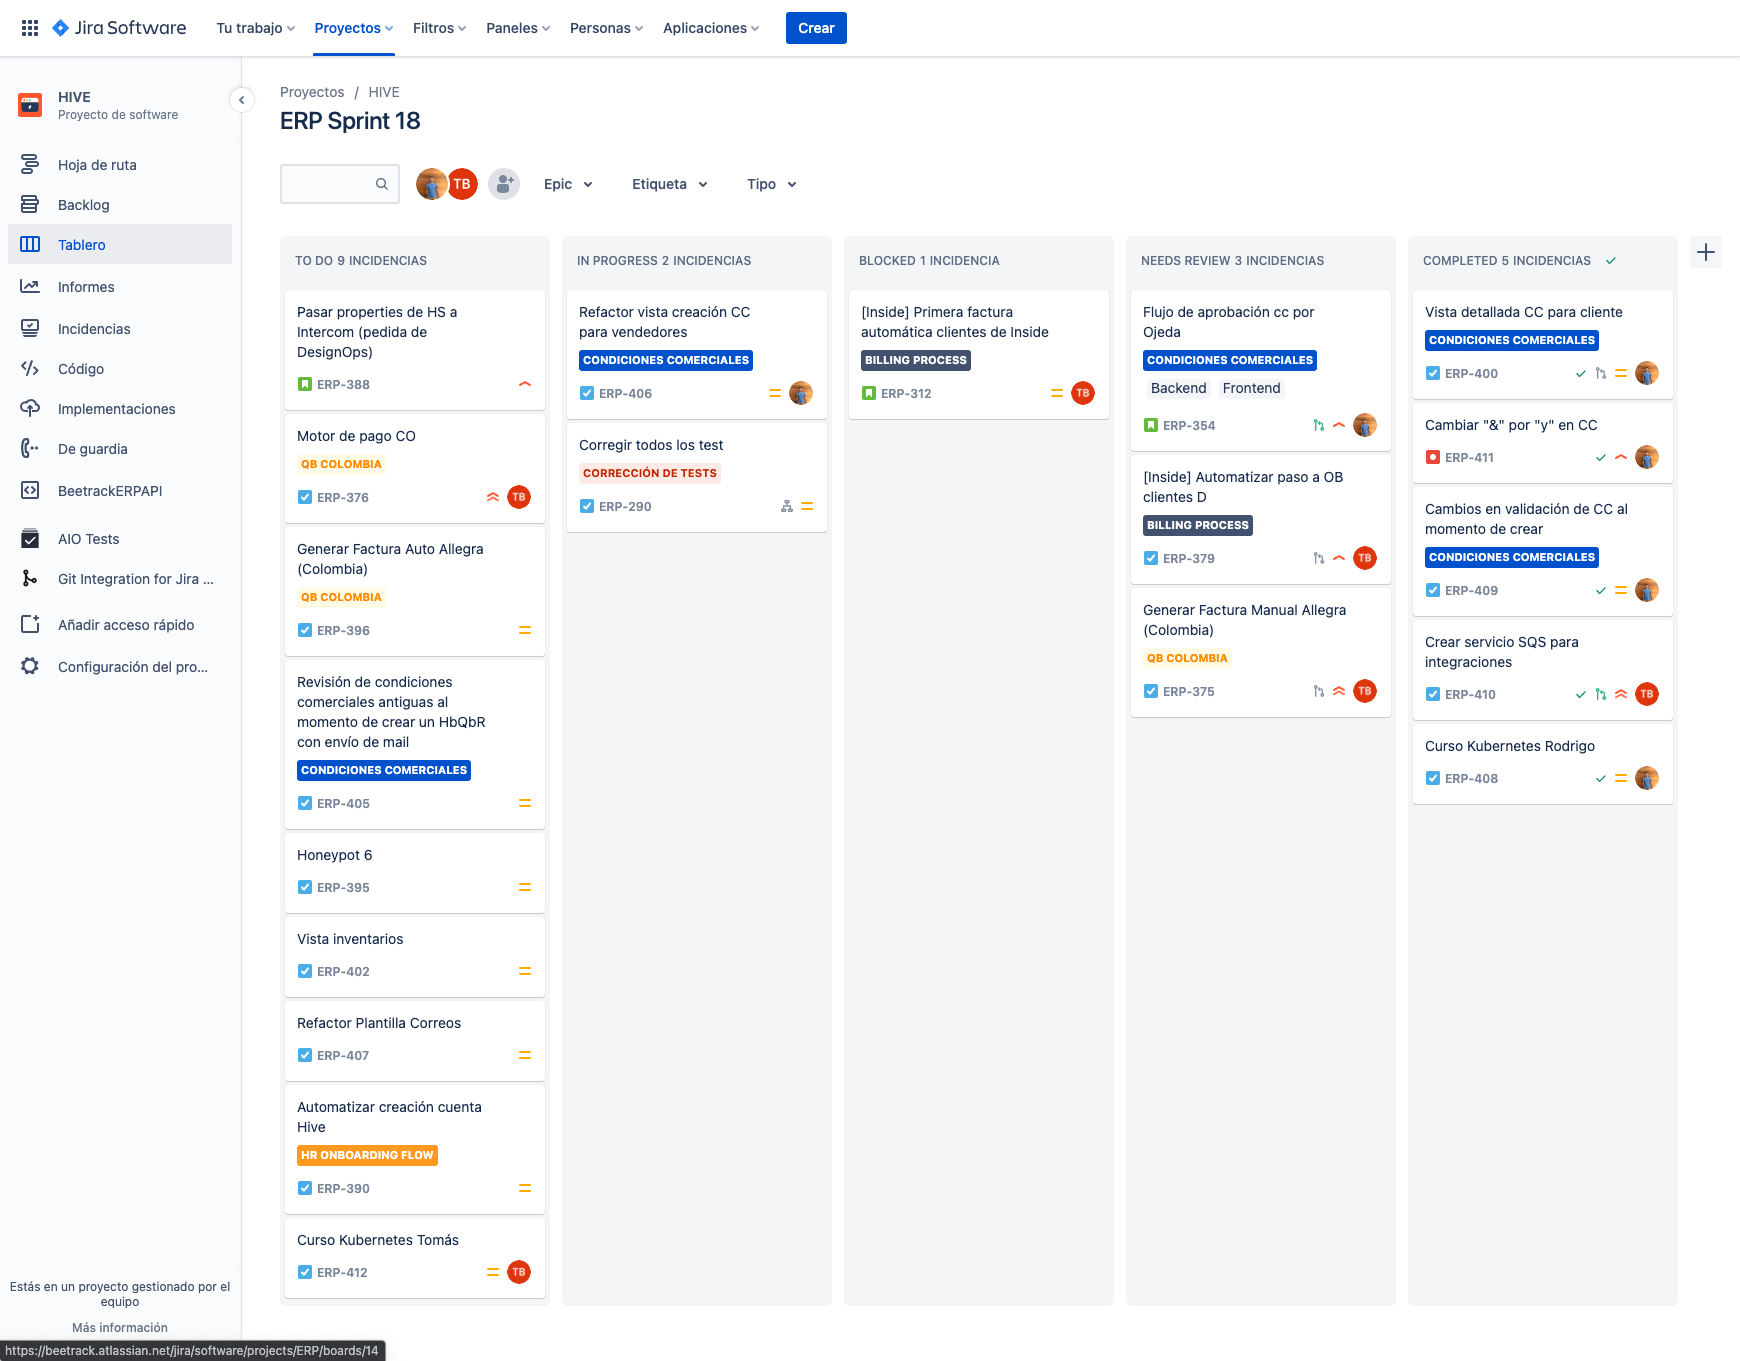
\includegraphics[width=0.75\linewidth]{figures/jira.png}
        \caption{Tablero \textit{Kanban} utilizado en el proyecto.}
        \label{fig:kanban}
    \end{figure}
    
    Debido a la cantidad de cambios que se deben realizar constantemente en el código, se requiere un versionamiento de este, por lo que se utiliza GitHub. Esta herramienta permite el uso de Git con \textit{Gitflow}. La principal ventaja de esta herramienta es que permite mantener diferentes versiones, como también utilizar un repositorio en donde se almacena el código en diferentes estados mediante \textit{branches}. Este uso de \textit{branches} o ``ramas'' permite mantener diferentes ambientes aislados uno del otro. El proyecto de \textit{Hive} cuenta con 3 ramas fijas, que nunca son eliminadas, \textit{master}, \textit{staging} y \textit{develop}. La primera rama es aquella que se encuentra en producción, es decir, es la que es visible para los usuarios finales, la segunda es un ambiente de pruebas (principalmente de estabilidad y de \textit{quality assurance}), y finalmente, la última es la rama de desarrollo, que es aquella en la cual se encuentra el código no probado por personas y que no se encuentra en ningún servidor de manera activa. 
    
    Cuando se quiere desarrollar una nueva funcionalidad, hacer correcciones o realizar cualquier tipo de cambio de código, la práctica es crear una nueva rama, hacer los cambios respectivos en el código, hacer una solicitud de cambio y revisión cruzada entre los miembros que tienen acceso al código mediante lo que se denomina un \textit{pull request}, para finalmente integrar los cambios a la rama principal una vez que los cambios hayan sido aprobados por los otros miembros del equipo. En la figura \ref{fig:gitflow_diagram} se puede ver cómo se vería un diagrama de un flujo en Git.
    
    \begin{figure}
        \centering
        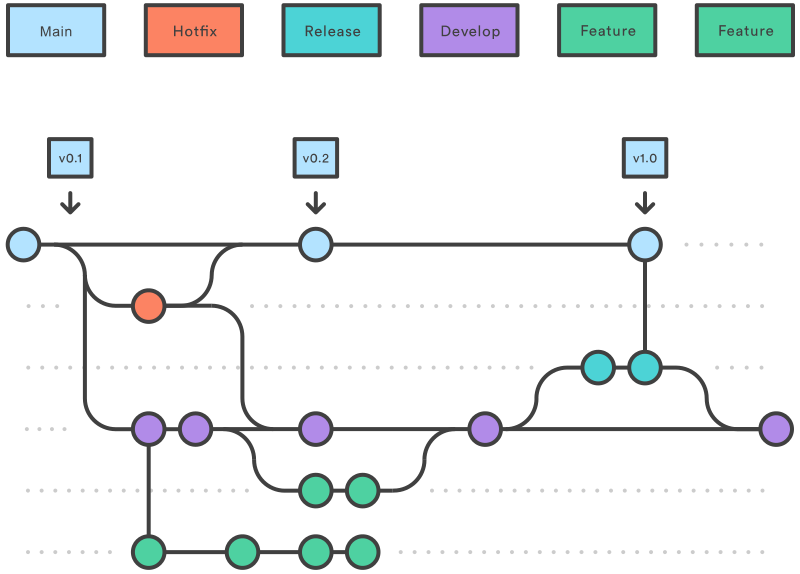
\includegraphics[width=0.65\linewidth]{figures/gitflow.png}
        \caption{\textit{Gitflow} \protect\cite{gitflow_diagram}.}
        \label{fig:gitflow_diagram}
    \end{figure}
    
    Finalmente, dentro de la empresa se utilizan procesos de integración continua, los cuales consisten en escritura de código que permite la puesta en producción del código que se subió a GitHub de manera automatizada en servidores remotos. En particular, se utiliza el SaaS Circle CI como intermediario. El flujo de integración continua, normalmente, comienza al subir el código a la rama \textit{master} o \textit{staging}, lo que gatilla una acción en los servidores de Circle CI, que descargan el código recién subido, corren pruebas sobre este, verifican su integridad, y finalmente compilan el código para subirlo a los servidores remotos especificados. La importancia de estas automatizaciones dentro de las metodologías de trabajo es que en el minuto en que estas automatizaciones fallan se despliegan alertas que permiten evitar que los servidores en producción se caigan por errores no previstos, sumado al hecho de que se permite ahorrar tiempo con tareas sistemáticas y bien establecidas.
    

\section{Tecnologías utilizadas}

    El ERP de la empresa se basa en una arquitectura que separa de manera lógica los componentes. \textit{Hive} mismo tiene una separación entre \textit{frontend} y \textit{backend}, el primero correspondiendo a todo lo que concierne a la forma de visualizar e interactuar con la aplicación, mientras que el segundo se encarga de todas las operaciones y lógica de negocio de la aplicación, junto con sus interacciones. Estas dos partes se comunican mediante varios \textit{endpoints} a través de una API (\textit{Application Programming Interface}) que el \textit{backend} expone. 
    
    Por un lado, una API es un conjunto de definiciones y protocolos que se utiliza para desarrollar e integrar el software de las aplicaciones \cite{redhat_api}. Por otro lado, un \textit{endpoint} es una URL (\textit{Uniform Resource Locator}), o punto de acceso, mediante el cual una aplicación, o API, puede utilizar para obtener recursos y comunicarse con otra aplicación. En el caso del ERP, los \textit{endpoints} cuentan con una capa de seguridad para evitar accesos indeseados de aplicaciones no verificadas, teniendo que identificarse con un JWT (\textit{JSON Web Token}), el cual funciona como llave de acceso para la API y el \textit{backend}. En particular, se utiliza la librería Devise para generar los JWT que son utilizados por la aplicación \textit{frontend} y son únicos por sesión de usuario.
    
    El \textit{backend} de la aplicación está desarrollado en el lenguaje Ruby con el \textit{framework} Rails, por lo que se denomina \textit{Ruby on Rails} (o RoR). Este \textit{framework} permite construir aplicaciones rápidamente que sigan los patrones de diseño de ingeniería de \textit{software} de manera muy simple y que puedan escalar rápidamente. El patrón más utilizado por este \textit{framework} es el MVC (Modelo Vista Controlador), el cual divide a la aplicación en las tres partes mencionadas. En primer lugar, el modelo es un conjunto de clases que representan la información del mundo real que el sistema debe procesar. En segundo lugar, las vistas son el conjunto de clases que se encargan de mostrar al usuario la información contenida en el modelo. Finalmente, el controlador es un objeto que se encarga de dirigir el flujo del control de la aplicación debido a mensajes externos, como datos introducidos por el usuario u opciones del menú seleccionadas por él \cite{mvc_architecture}.
   
   En particular, para almacenar los datos de largo plazo del modelo se utiliza una base de datos con un motor PostgreSQL (o PSQL). Cabe mencionar que no todos los datos se almacenan en este tipo de memoria y que no todas las operaciones se pueden realizar con esta. Es por lo anterior que también se hace uso de Sidekiq, una librería que permite la ejecución de tareas de manera asíncrona y/o en una fecha determinada mediante el almacenamiento de los datos necesarios en memoria \textit{caché}, para lo que se utiliza el motor Redis.
   
   Dada la naturaleza del ERP, como se mencionó anteriormente, este interactúa con otros servicios de dos maneras. Por un lado, para el servicio de condiciones comerciales, proyecto que el alumno realizó, se utiliza GraphQL, mientras que para el resto de los servicios, tales como Hubspot y Quickbooks, entre otros, se utiliza APIs REST. Una API REST es una API que se ajusta a los principios de diseño de REST, un estilo de arquitectura también denominado transferencia de estado representacional \cite{ibm_api_rest}. Este estilo es uno de los más populares para hacer APIs, pero es menos flexible al compararlo con GraphQL. Este último, es un lenguaje de consultas y servicio para APIs que prioriza el entregar a los consumidores exactamente la información solicitada y no más que eso. El principio de este lenguaje es hacer las APIs más flexibles, rápidas y posicionarse como alternativa a REST \cite{def_graphql}.
   
   El \textit{frontend} de \textit{Hive} está desarrollado en JavaScript con el \textit{framework} React. El código está construido sobre el principio de componentes reusables en las diferentes partes de la aplicación de manera de seguir el principio DRY (\textit{Don't Repeat Yourself}). Dado que el \textit{frontend} es aquel con el cual los usuarios interactúan, este requiere estilo, el cual está dado por el \textit{desing system, Honeypot}, de Beetrack. Este sistema de diseño es utilizado en todas las aplicaciones de la empresa de manera de que se pueda mantener una consistencia visual y de usabilidad entre las diferentes partes que componen los \textit{softwares} que se producen dentro de la empresa. En particular, este \textit{design system} abarca elementos como paleta de colores, diseños visuales de botones, formularios y componentes, entre otros, mientras que al mismo tiempo se tratan como paquetes prehechos, lo que permite reutilizarlos.
   
   
   En último lugar, tanto la aplicación de \textit{Hive} como el servicio de condiciones comerciales están alojadas en GKE (Google Kubernetes Engine). Este servicio permite mantener las aplicaciones mediante imágenes compiladas de Docker en servidores que son fácilmente escalables tanto vertical como horizontalmente, mientras que al mimso tiempo se encarga de los procedimientos para generar estos servidores y que se coordinen entre ellos. Otra ventaja que provee GKE es la facilidad para poder volver imágenes que ya no se encuentran en uso en el caso de que ocurra algún error, lo que permite aumentar la disponibilidad del servicio entregado. En la figura \ref{fig:arquitectura} se puede ver la arquitectura con la cual el alumno trabajó.
   
   \begin{figure}
       \centering
       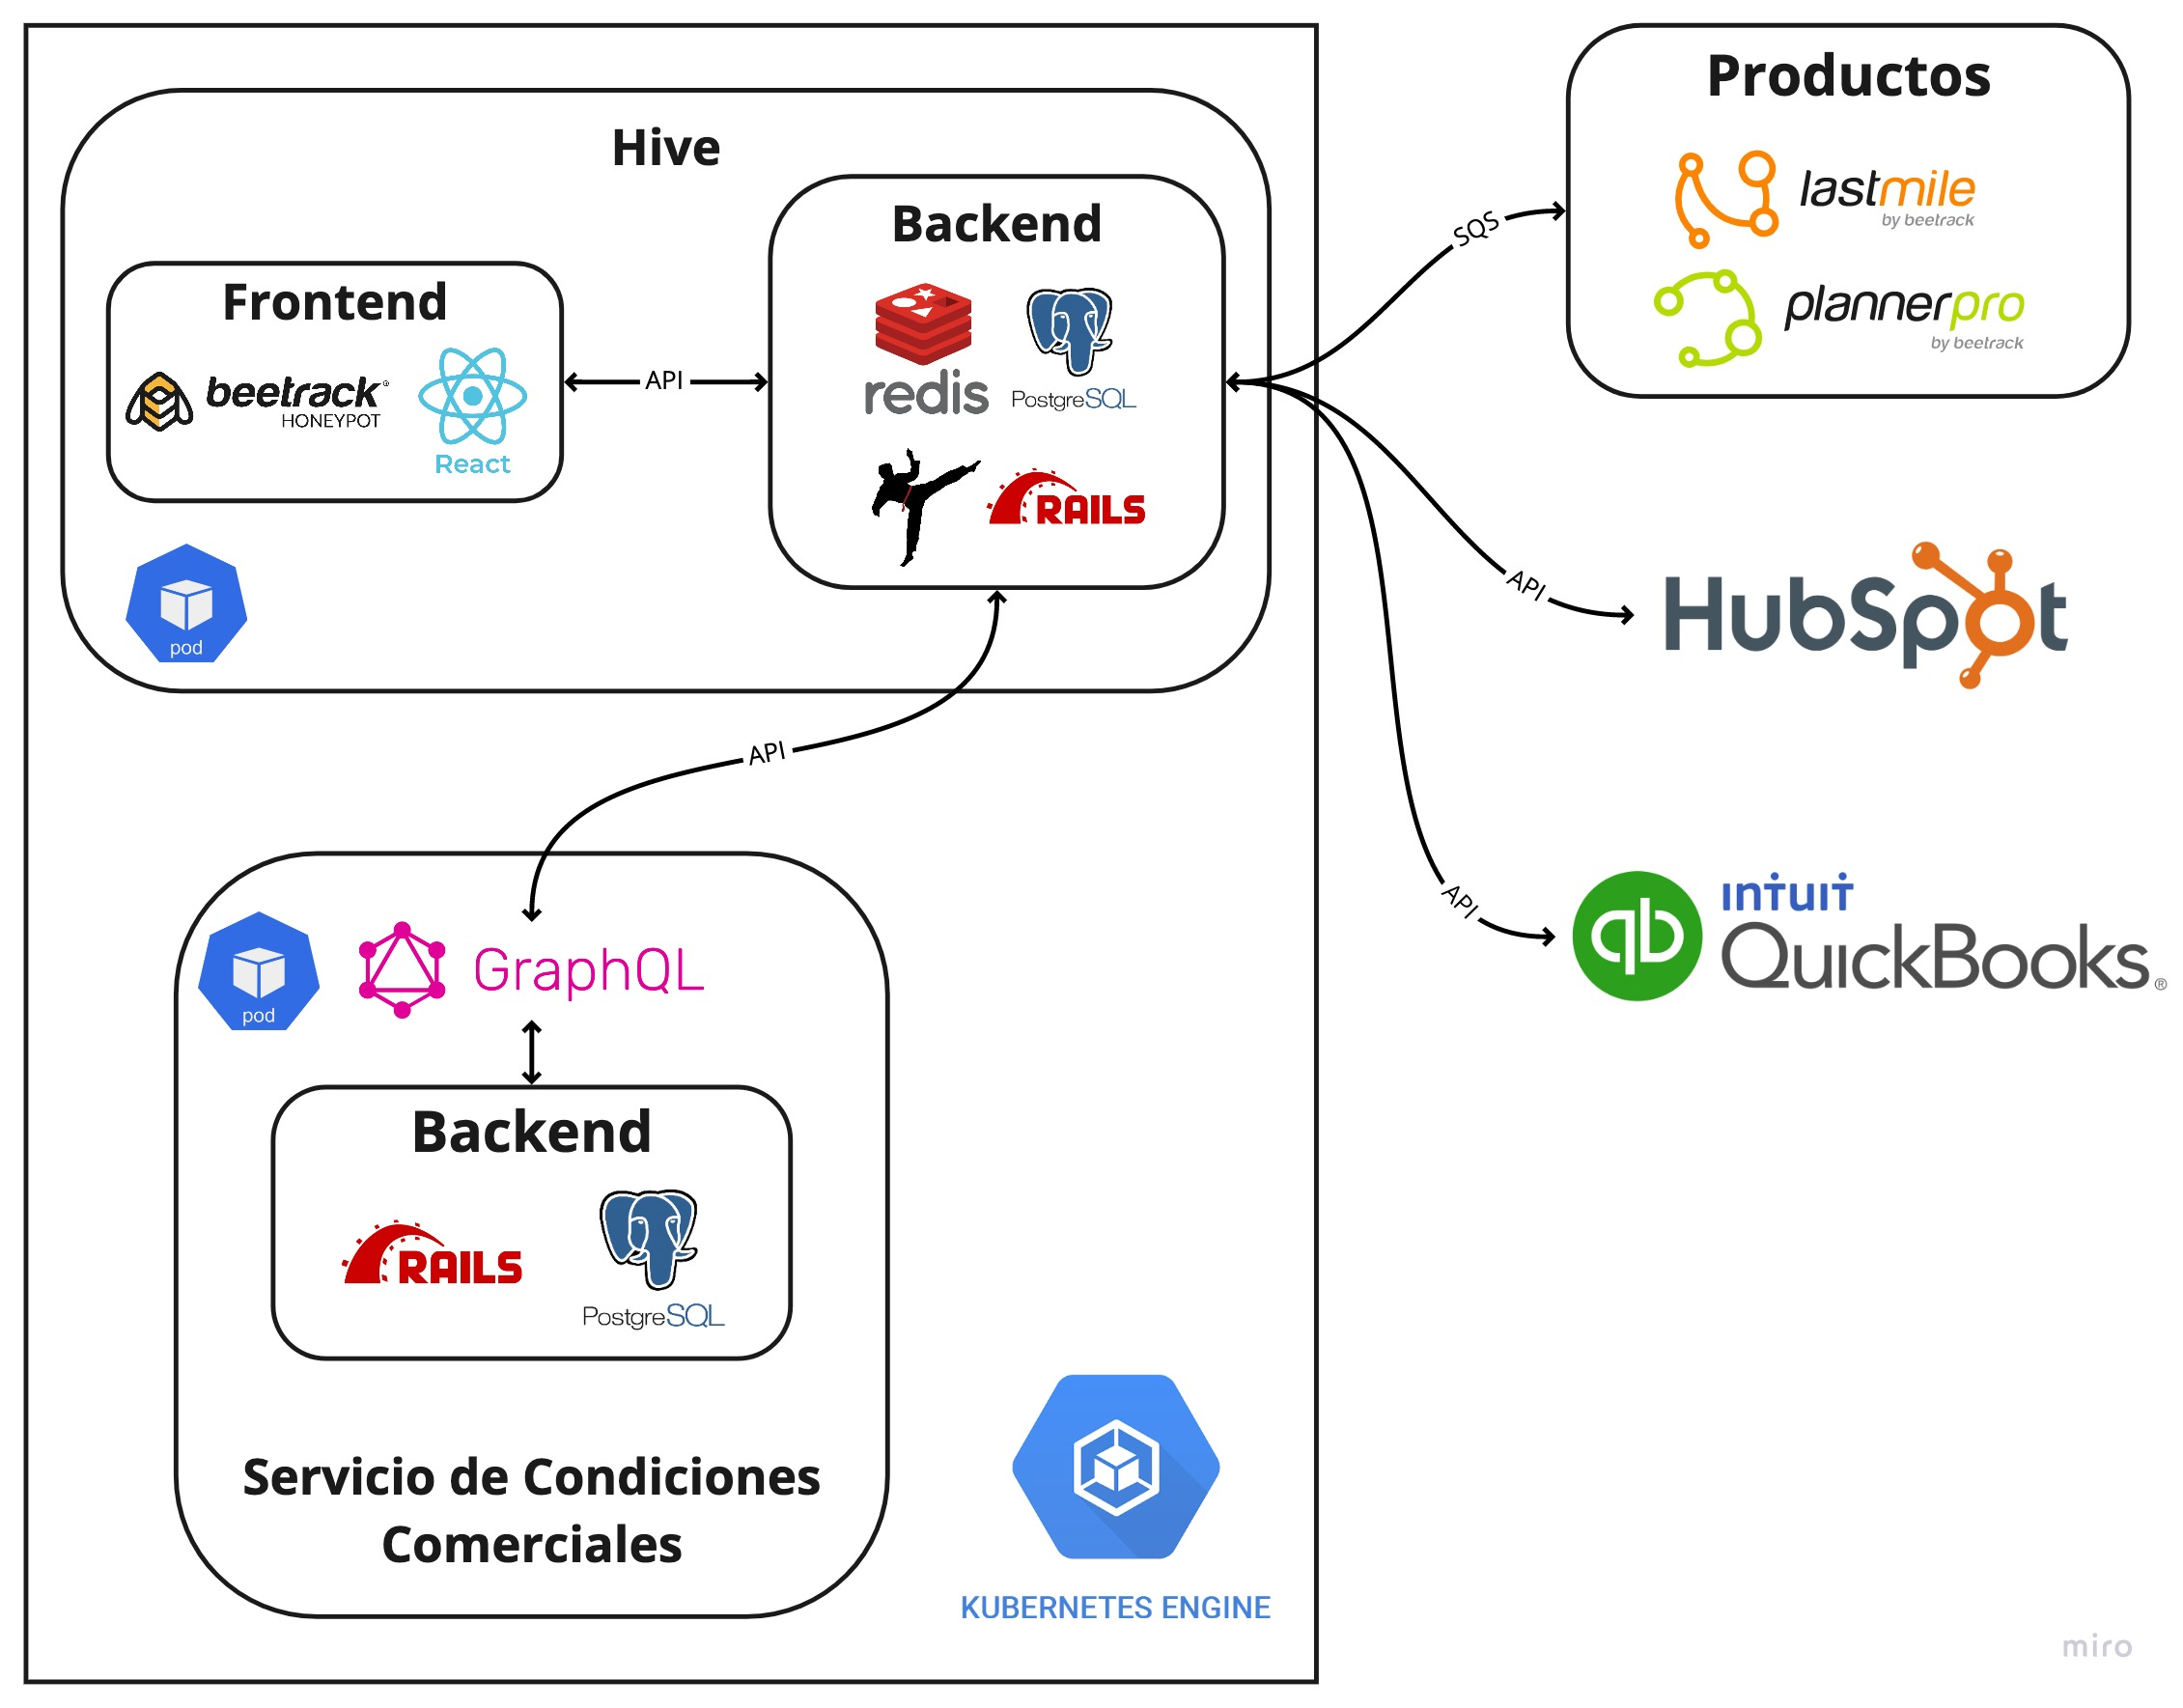
\includegraphics[width=0.75\linewidth]{figures/arquitectura.jpg}
       \caption{Diagrama de tecnologías y arquitectura.}
       \label{fig:arquitectura}
   \end{figure}
   
   
% Por último, se utiliza el servicio de Kubernetes de Google para mantener
% alojada la aplicación web. Este servicio permite a través de contenedores de Docker
% mantener la aplicación web de una forma que es fácilmente replicable en caso de
% necesitar más potencia de cómputo (Nieto, 2021). Otra ventaja del uso de Kubernetes
% es la facilidad para volver a estados anteriores de los contenedores en caso de algún
% tipo de error. En la figura 2.2, se puede apreciar el esquema de la arquitectura utilizada
% dentro de Hive y como interactúa con otros servicios externos.

\chapter{Aumento de cobertura de pruebas e integración continua} \label{testing}
\textit{}\section{Objetivos y contextualización}

  Una práctica muy utilizada dentro del desarrollo de proyectos grandes de \textit{software} es el uso de pruebas unitarias y de integración de los diferntes componentes de la aplicación sobre la que se trabaja. Esta práctica tiene dos objetivos principales: primero el poder tener seguridad de que el código escrito efectivamente cumple el propósito para el cuál fue programado, y en segundo lugar, el tener la seguridad de que al cambiar una parte del código, este siga cumpliendo su función original. En la práctica, el segundo punto es sumamente útil al momento de realizar cambios al \textit{codebase} existente, dado que se quiere seguir teniendo la misma funcionalidad, pero cambiando el código interno, en lo que se conoce como \textit{refactor} y mediante las pruebas se puede tener la seguridad de que todo siga en orden después de haber realizado los cambios. 
  
  En este sentido, es paradójico que, una empresa que se dedica a producir \textit{software}, no haga pruebas rigurosas de sus desarrollos internos. Es por lo anterior, que el alumno le sugirió a su superior, Nicolás Kipreos, aumentar significativamente la cantidad de pruebas que existen para el ERP, junto con la integración de estas a un flujo de integración continua de manera de que se pudiese tener una mayor seguridad y cofianza al momento de poner en producción el nuevo código.

  El pricipal beneficio que el área de \textit{TechOps} tendría mediante la implementación de una mayor cantidad de pruebas y la integración de estas pruebas a un flujo de integración continua serían tres. En primer lugar, el tener la seguridad de que el código efectivamente hace lo que se pretende que haga, en segundo lugar el saber que el código no se caerá de manera inesperada frente a un cambio y, en tercer lugar, el forzar a que el código sea probado antes de ser puesto en producción \cite{ibm_testing}, evitando que los errores lleguen a los usuarios de la plataforma.

  La meta que se estableció por parte del alumno fue de llegar a una cobertura mínima de 60\% sin pruebas fallidas, junto con el forzar a que el flujo de \textit{deployment} de la aplicación fallara en caso que alguna prueba no funcionara en Circle CI.

\section{Desarrollo}

  En RoR, se hace uso de la herramienta RSpec para hacer el \textit{testing} de manera automatizada y poder correr las pruebas correspondientes. En el caso de \textit{Hive}, cuando el alumno llegó al proyecto, este tenía una cobertura de 35,44\%. Esto quiere decir que solamente una de cada tres líneas de todo el código existente en \textit{Hive} era ejecutada y probada. Cabe mencionar también que aproximadamente un tercio de las pruebas que existían fallaban, es decir, el código no cumplía con las pruebas que se relizaban sobre el, teniendo un comportamiento diferente al esperado.
   En la figura \ref{fig:testing_original} se puede observar el estado inicial de la cobertura de las pruebas del ERP.

  \begin{figure}[H]
    \centering
    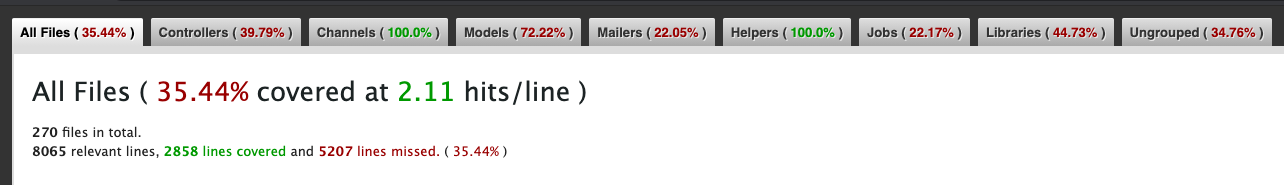
\includegraphics[width=\linewidth]{figures/testing/testing_original.png}
    \caption{Cobertura inicial del ERP (captura tomada el 3 de agosto de 2021).}
    \label{fig:testing_original}
  \end{figure}

  Dado que \textit{Hive}, en agosto, tenía aproximadamente 8000 líneas de código, el proceso del aumento de la cobertura del \textit{testing} comenzó mediante la revisión y mapeo de todos los archivos existentes y su estado de cobertura de pruebas. En otras palabras, se revisó todo el código fuente del ERP para saber cuáles archivos eran cubiertos por las pruebas automatizadas, cuáles no y cuáles requerían correcciones. De esta manera se podía ver con claridad en qué partes se tenía que enfocar los esfuerzos de trabajo y se podía saber cuáles archivos era más críticos de revisar y probar.

  El alumno realizó el mapeo de los archivos junto a Tomás Burotto y dejaron los registros en una sección especial de Jira. Esta documentación se organizó por secciones y subsecciones de archivos y carpetas, siguiendo la misma estructura de \textit{Hive}. Una vez que se transpasaron todos los archivos, se procedió a ponerles etiquetas del estado en que se encontraban, tal como se puede observar en la figura \ref{fig:mapeo_tests}.
  
  \begin{figure}
    \centering
    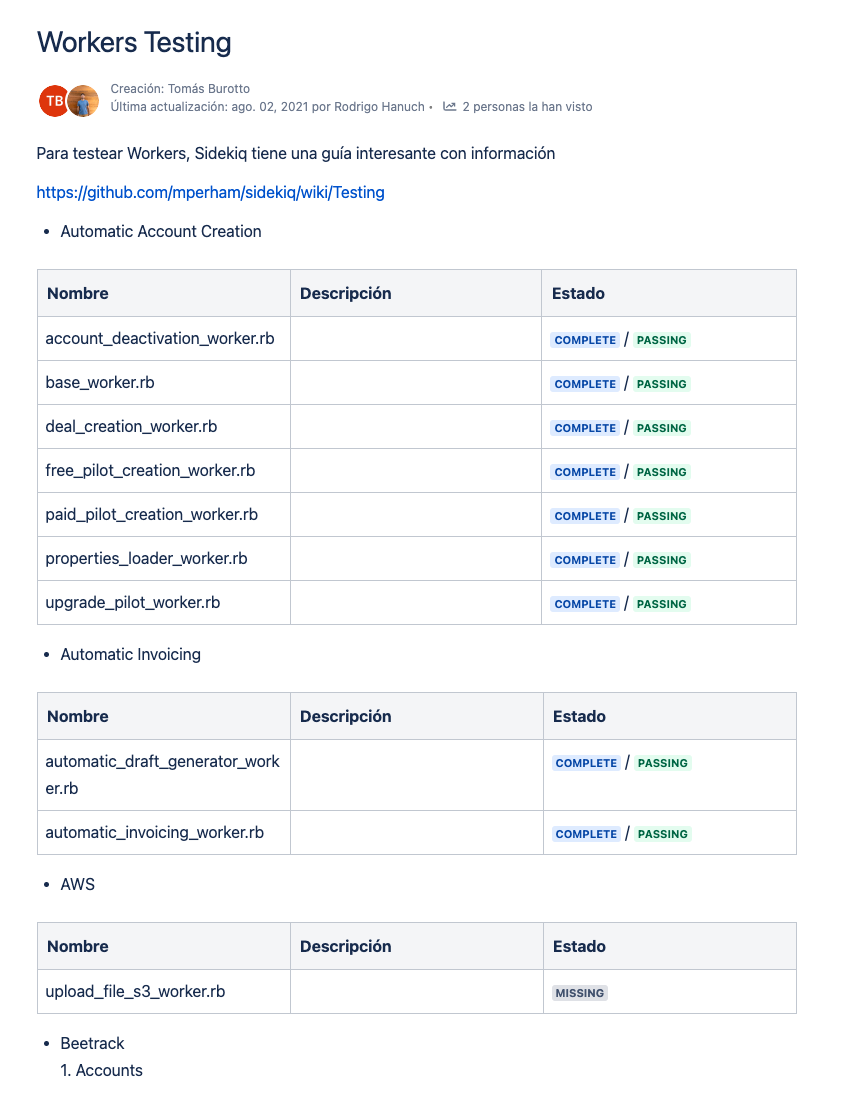
\includegraphics[width=0.75\linewidth]{figures/testing/mapeo_tests_existentes.png}
    \caption{Clasificación y etiquetado de los diferentes archivos y sus estados.}
    \label{fig:mapeo_tests}
  \end{figure}

  Se decidió tener 3 estados para la cobertura: ``\textit{complete}'', en el cual 100\% de las líneas correspondientes del archivo eran cubiertas, ``\textit{partial}'', para indicar que no todas las líneas del archivo eran cubiertas y ``\textit{none}'', para indicar que el archivo de pruebas existía, pero ninguna línea era cubierta.
  
  Por otro lado, también existían 3 etiquetas para el estado en que se econtraban las pruebas: ``\textit{passing}'' que aplicaba en caso de que todos los \textit{test} estuviesen pasando, ``\textit{failing}'' para indicar que una o más pruebas fallaban y ``\textit{skipped}'', que indicaba que una o más de las pruebas eran saltadas. Finalmente, se hizo una etiqueta adicional llamada ``\textit{missing}'' que se aplicó en el caso de que no existiese el archivo de pruebas correspondiente.
  
  Una vez que el alumno tuvo visibilidad del estado del \textit{testing} de la aplicación, este procedió a programar las pruebas automatizadas del código existente. Esto implicó el crear los archivos faltantes para el código que no era probado y leer el código existente, de manera de poder realizar pruebas adecuadas y no simplemente hacer pruebas que pasaran con cualquier resultado. La principal ventaja de realiazr pruebas muy detalladas es que permite tener un desgolse muy granular de qué falla en caso de que algo no funcione dentro del sistema, de manera de que se pueda corregir rápidamente y sin mayor conflicto. En particular, el alumno se enfocó en realizar pruebas automatizadas para la sección de \textit{workers}. El principal motivo del enfoque en estos archivos es debido a que los \textit{workers}, son procesos que corren de manera asíncrona del código principal del ERP y que son automatizaciones sensibles, como, por ejemplo, la generación de facturas y pre-facturas de manera automática, notificación a usuarios internos de la empresa, y cambios de estados en los contratos y datos de Hubspot, los cuales son vistos por los vendedores.

  Luego de que el estudiante cumpliera la meta establecida, este procedió a la siguiente tarea, la cual consistió en el cambió del \textit{deployment code} de Circle CI. El flujo de puesta en producción de Circle CI funciona mediante la declaración de pasos a seguir al momento de hacer un \textit{code deploy}. Previamente, la implementación de este código solamente contenía la compilación de los archivos y subida de estos a GKE. Para poder realizar la automatización de las pruebas en este entorno, se tuvo que levantar una imagen virtual de PostgreSQL en el contenedor de Circle CI y hacer que no finalizara su conexión luego de que se construyera, esto dado que para correr RSpec (el comando utilizado para correr las pruebas), se tiene que tener entradas en las bases de datos y para esto se tiene que tener una conexión abierta.

  El código que el alumno escribió para el flujo de Circle CI fue hecho de tal manera de que tuviese 2 pasos: en primer lugar las pruebas automatizadas, y luego, en caso de que la primera etapa fuese exitosa, el segundo paso, el \textit{deploy} y compilación del código para ser puesto en producción. Lo anterior permite que se pueda cortar el flujo en caso de que el primer paso falle, liberando antes los servidores que se utilizan de manera común en Beetrack para hacer \textit{deployment} tanto de los productos principales, como del \textit{software} interno de la emprsa. En la figura \ref{fig:flujo_circle_ci} se puede observar tanto el cambio de un flujo único sin pruebas automatizadas a uno con pruebas y el hecho de que cuando falla RSpec, el flujo se corta de inmediato, evitando el poner código defectuso en producción.

  \begin{figure}
    \centering
    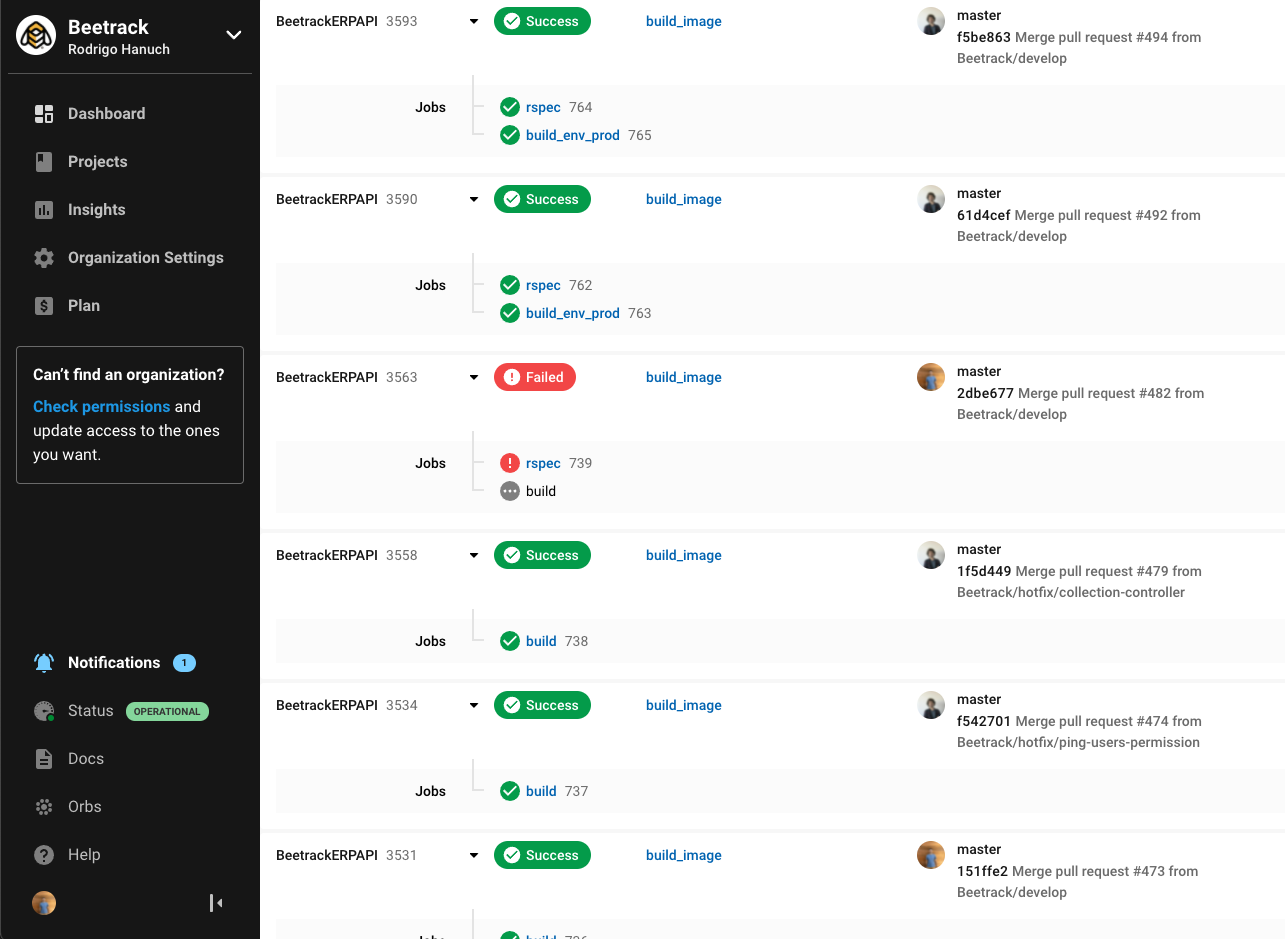
\includegraphics[width=\linewidth]{figures/testing/circle_ci_flow.png}
    \caption{Cambio en flujos de Circle CI y falla de \textit{RSpec} previa a la puesta en producción del código.}
    \label{fig:flujo_circle_ci}
  \end{figure}

\section{Resultados}

  Los principales resultados obtenidos de este proyecto fueron superiores a los propuestos originalmente. En particular se logó lo siguiente:
  
  \begin{enumerate}
    \item Cobertura de final de 64,04\% en \textit{Hive}.
    
    Se logró una cobertura de un 64,04\% del ERP, tal como se puede ver en la figura \ref{fig:testing_final}. Esto fue posible mediante la \textbf{simulación} de la ejecución de código previo a su puesta en producción y la aplicación de \textbf{conocimientos avanzados} de \textit{testing} para el \textit{framework} de RoR. Sumado a esto, también se tuvo extremo cuidado al momento de desarrollar las pruebas, evitando el escribir contraseñas o información sensible en estos mediante el uso de las herramientas proveídas por Rails, \textbf{cumpliendo con restricciones técnicas y éticas} para evitar que estas sean filtradas de manera pública a internet.
    
    \begin{figure}[H]
      \centering
      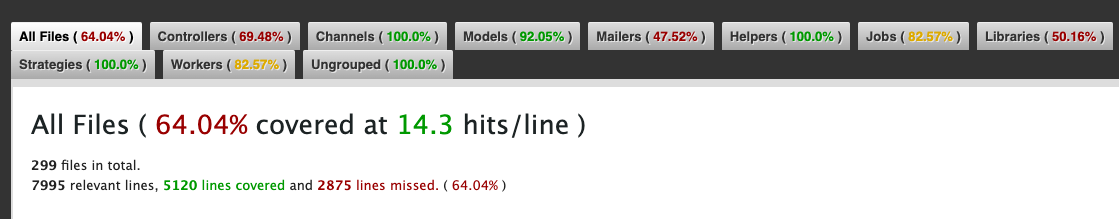
\includegraphics[width=\linewidth]{figures/testing/testing_final.png}
      \caption{Cobertura final del ERP (captura tomada el 15 de noviembre de 2021).}
      \label{fig:testing_final}
    \end{figure}

    \item Escritura de más de 2800 líneas de pruebas automatizadas.
    
    El incremento de la cobertura se logró mediante la escritura o modificación de 115 archivos con un total de 2816 líneas de código nuevas dedicadas exclusivamente a la automatización del proceso de pruebas, lo cual se puede ver en la figura \ref{fig:testing_file_commits}.

    \begin{figure}[H]
      \centering
      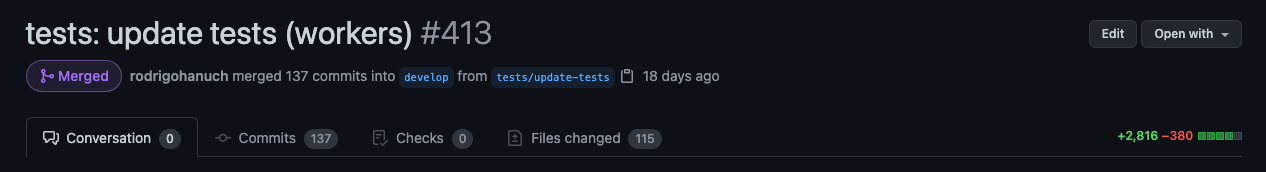
\includegraphics[width=\linewidth]{figures/testing/testing_file_commits.png}
      \caption{Archivos modificados y generados durante creación de nuevas pruebas.}
      \label{fig:testing_file_commits}
    \end{figure}

    \item Implementación de flujo de integración continua con pruebas automatizadas.
    
    La implementación del flujo de pruebas automatizadas en Circle CI tiene como principal resultado el incremento en confiabilidad del código escrito, y, por lo tanto, la disminución del \textit{downtime} generado por líneas no probadas para el equipo \textit{TechOps} y para la aplicación de \textit{Hive}. Sumado a lo anterior, esta implementación también consideró un flujo con menor cantidad de código al reescribir, en gran parte, los comandos que generaban los \textit{deployments} a GKE, reutilizando código y haciéndolo más legible al aplicar \textbf{patrones de diseño de \textit{software}} y eliminando muchos \textit{code smells} (antipatrones de diseño, que ocurren cuando el código no sigue estándares y que pueden indicar problemas más profundos \cite{code_smells}).

  \end{enumerate}
 

\chapter{Servicio de Condiciones Comerciales} \label{servicio_cc}
\section{Objetivos y contextualización}

  Actualmente, la empresa tiene más de 700 clientes activos, cada uno con diferentes contratos, o condiciones comerciales, y se utiliza un archivo de Excel para mantener estas condiciones actualizadas. Al mismo tiempo, este excel también contiene la forma en que se calculan los costos totales por el uso del servicio para cada cliente. Similar a lo que ocurría con la falta de pruebas automatizadas, también resulta curioso el hecho de que Beetrack, siendo una empresa SaaS y teniendo su propio ERP, utilice esta plantilla para calcular cuánto cobrarle a los clientes. Es por lo anterior que decidió crear un servicio especializado en el almacenamiento y cálculo de estas condiciones comerciales, y cuyo único propósito fuese resolver el problema de cómo calcular los costos por cliente y poder almacenar los modelos que representaran los contratos generados con estos.
  
  Uno de los puntos más cruciales sobre este servicio y su contexto es el hecho de que ya se había intentado dos veces algo similar. El primer intento fue mediante un desarrollo interno en el ERP, el cual no tuvo los resultados esperados en términos de precisión al momento de facturar y se concluyó que no era responsabilidad de \textit{Hive} como tal tener esta información. El segundo intento fue la migración de estos planes a un proyecto que, en su minuto, se encontraba en fase \textit{beta} en Hubspot, en el cual se prometía poder tener la información siempre actualizada. Finalmente terminó ocurriendo lo mismo que en el primer intento, pero con peor precisión al momento de facturar de manera automática, entregando, en el mejor de los casos, una precisión de 43\%.

  Teniendo en consideración los requisitos y los resultados anteriores, los objetivos principales del proyecto fueron dos. El primer objetivo, fue construir un modelo lo suficientemente flexible como para poder abarcar los diferentes tipos de ventas que los vendedores realizan, tanto para productos como servicios. El segundo objetivo fue el programar un servicio de resolución comercial, o calculadora, que fuese, nuevamente, lo suficientemente flexible como para poder abarcar el modelo, pero que al mismo tiempo no necesitara información contextual más allá del uso para saber cuánto cobrarle a cada cliente, mientras que al mismo tiempo entregaba glosas prehechas por producto.

  El equipo de Operaciones decidió no acoplar este proyecto a \textit{Hive} de manera de evitar el cruce indebido de información y para así poder mantener las ideas aisladas y para así comenzar a tener una arquitectura de sistemas distribuidos en base a servicios. Lo anterior sumado al hecho de que el se prevee que, eventualmente, otros servicios y productos de la empresan, tales como el \textit{Customer Portal}, consuman los recursos expuestos por este servicio de manera de que los clientes también puedan saber cuánto se les cobrará o el nivel de costo que tienen para un día determinado del mes. Como se puede ver en la figura \ref{fig:arquitectura}, del capítulo \ref{metodologias}, la arquitectura que se decidió utilizar es una en la cual el servicio de condiciones está aislada del ERP, mientras que al mismo tiempo no limita a que otro servicio pueda consumir la información del servicio nuevo, lo cual hubiese ocurrido en caso de haber escrito el código en \textit{Hive} dada su naturaleza monolítica.

\section{Desarrollo}

  \subsection{Modelamiento}

    El proceso de desarrollo del nuevo servicio de condiciones comerciales comenzó con un análisis de los diferentes planes existentes y que se encuentraban en uso en por parte de la empresa. Luego de realizar este análisis se definieron 4 modelos diferentes a nivel de base de datos que permitirían almacenar de manera flexible las condiciones con las cuales se les factura a los clientes. 
    
    En primer lugar se tiene el modelo del plan, en este se almacena la condición comercial como tal, junto con una descripción del uso que puede tener esta condición y el producto y moneda asociado a la condición. Dentro del campo ``\texttt{condition}'' se almacena el tipo de tramo y costos asociado que tendrá por ellos. Se decidió que se puede tener tres tipos de tramos diferentes: base, variable y por paso. A continuación se detalla cada tipo de tramo:
    \begin{enumerate}
      \item Tramo base: va desde cero unidades hasta la cantidad de unidades determinada con un costo fijo total por esas unidades. Solamente se puede tener un tramo de este tipo por plan.
      \item Tramo variable: funcionan mediante una definición de inicio a final del tramo en término de cantidad de unidades, con un precio unitario por la cantidad de unidades utilizadas. Se pueden tener entyre cero e infinitos tramos variables por plan.
      \item Tramo por pasos: se utilizan para poder representar los productos que se venden mediante paquetes, esto es especialmente útil para el servicio de correos en el cual se cobra mediante paquetes de 10.000 correos, siendo los primeros 10.000 gratis y los siguientes teniendo un costo de 1 UF por bolsa adicional. Este tipo de tramo es excluyente con los dos anteriores y solo se puede tener, el cual funciona de manera recurrente.
    \end{enumerate}
    
    Adicionalmente, el campo ``\texttt{condition}'' contiene dos variables utilizadas al momento de calcular el costo total al momento de generar la factura para un cliente. Estos se detallan a continuación:
    \begin{enumerate}
      \item \texttt{general\_minimum}: se utiliza para asegurar un monto mínimo de facturación del producto independiente del uso del cliente una vez que ya se haya calculado el costo por el uso que el cliente le haya dado al producto o servicio.
      \item \texttt{add\_base\_to\_variable}: se utiliza al momento de calcular el costo del uso del producto, y sirve para saber si el plan que se negoció con el cliente se entiende de manera de que se cobre sumando el costo base o utilizando el costo unitario del tramo variable en caso de aplicar.
    \end{enumerate}
    
    El esquema de información del campo ``\texttt{condition}'' se puede ver en la figura \ref{fig:cc_condition_schema}, mientras que en la figura \ref{fig:cc_pricing_chart} se puede observar una manera visual de entender el modelo de precios y condiciones comerciales de los clientes. Es importante mencionar que se hizo uno uso avanzados de RoR mediante la creación de artefactos de validación que permniten mantener los esquemas de datos establecidos en la figura \ref{fig:cc_condition_schema}. Al mismo tiempo, también se utilizó validación de los datos en si mismos, forzando a que siempre se tengan tramos positivos, sin sobrelape y que sean rangos acotados, de manera de que las condiciones siempre tengan las formas de la figura \ref{fig:cc_pricing_chart}.
    
    \begin{figure}
      \centering
      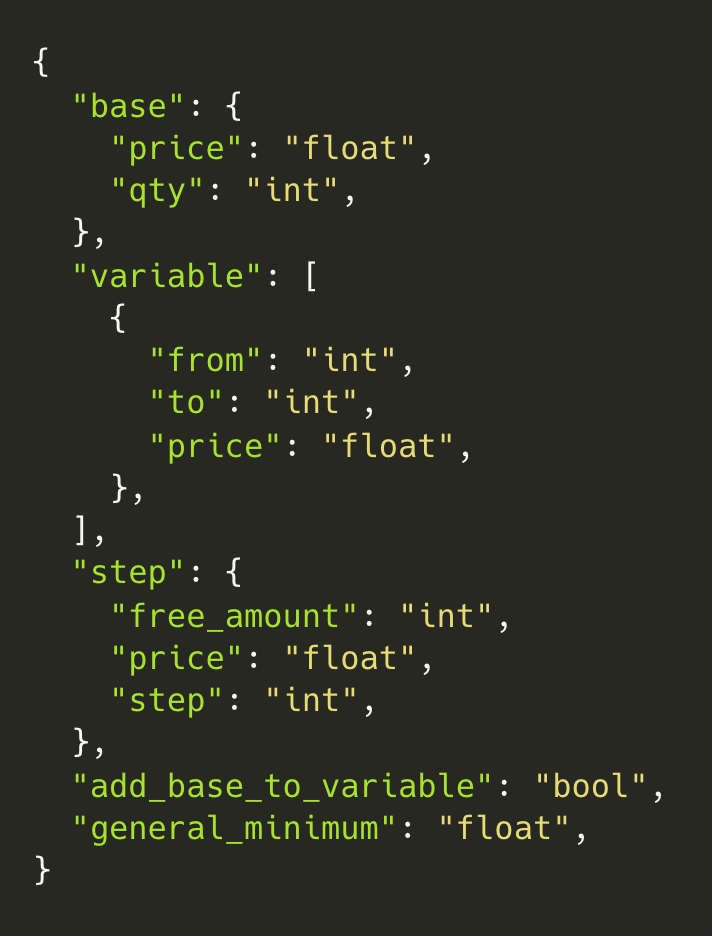
\includegraphics[width=0.4\linewidth]{figures/cc/cc_condition_schema.png}
      \caption{Esquema de información de condición comercial.}
      \label{fig:cc_condition_schema}
    \end{figure}

    \begin{figure}
      \centering
      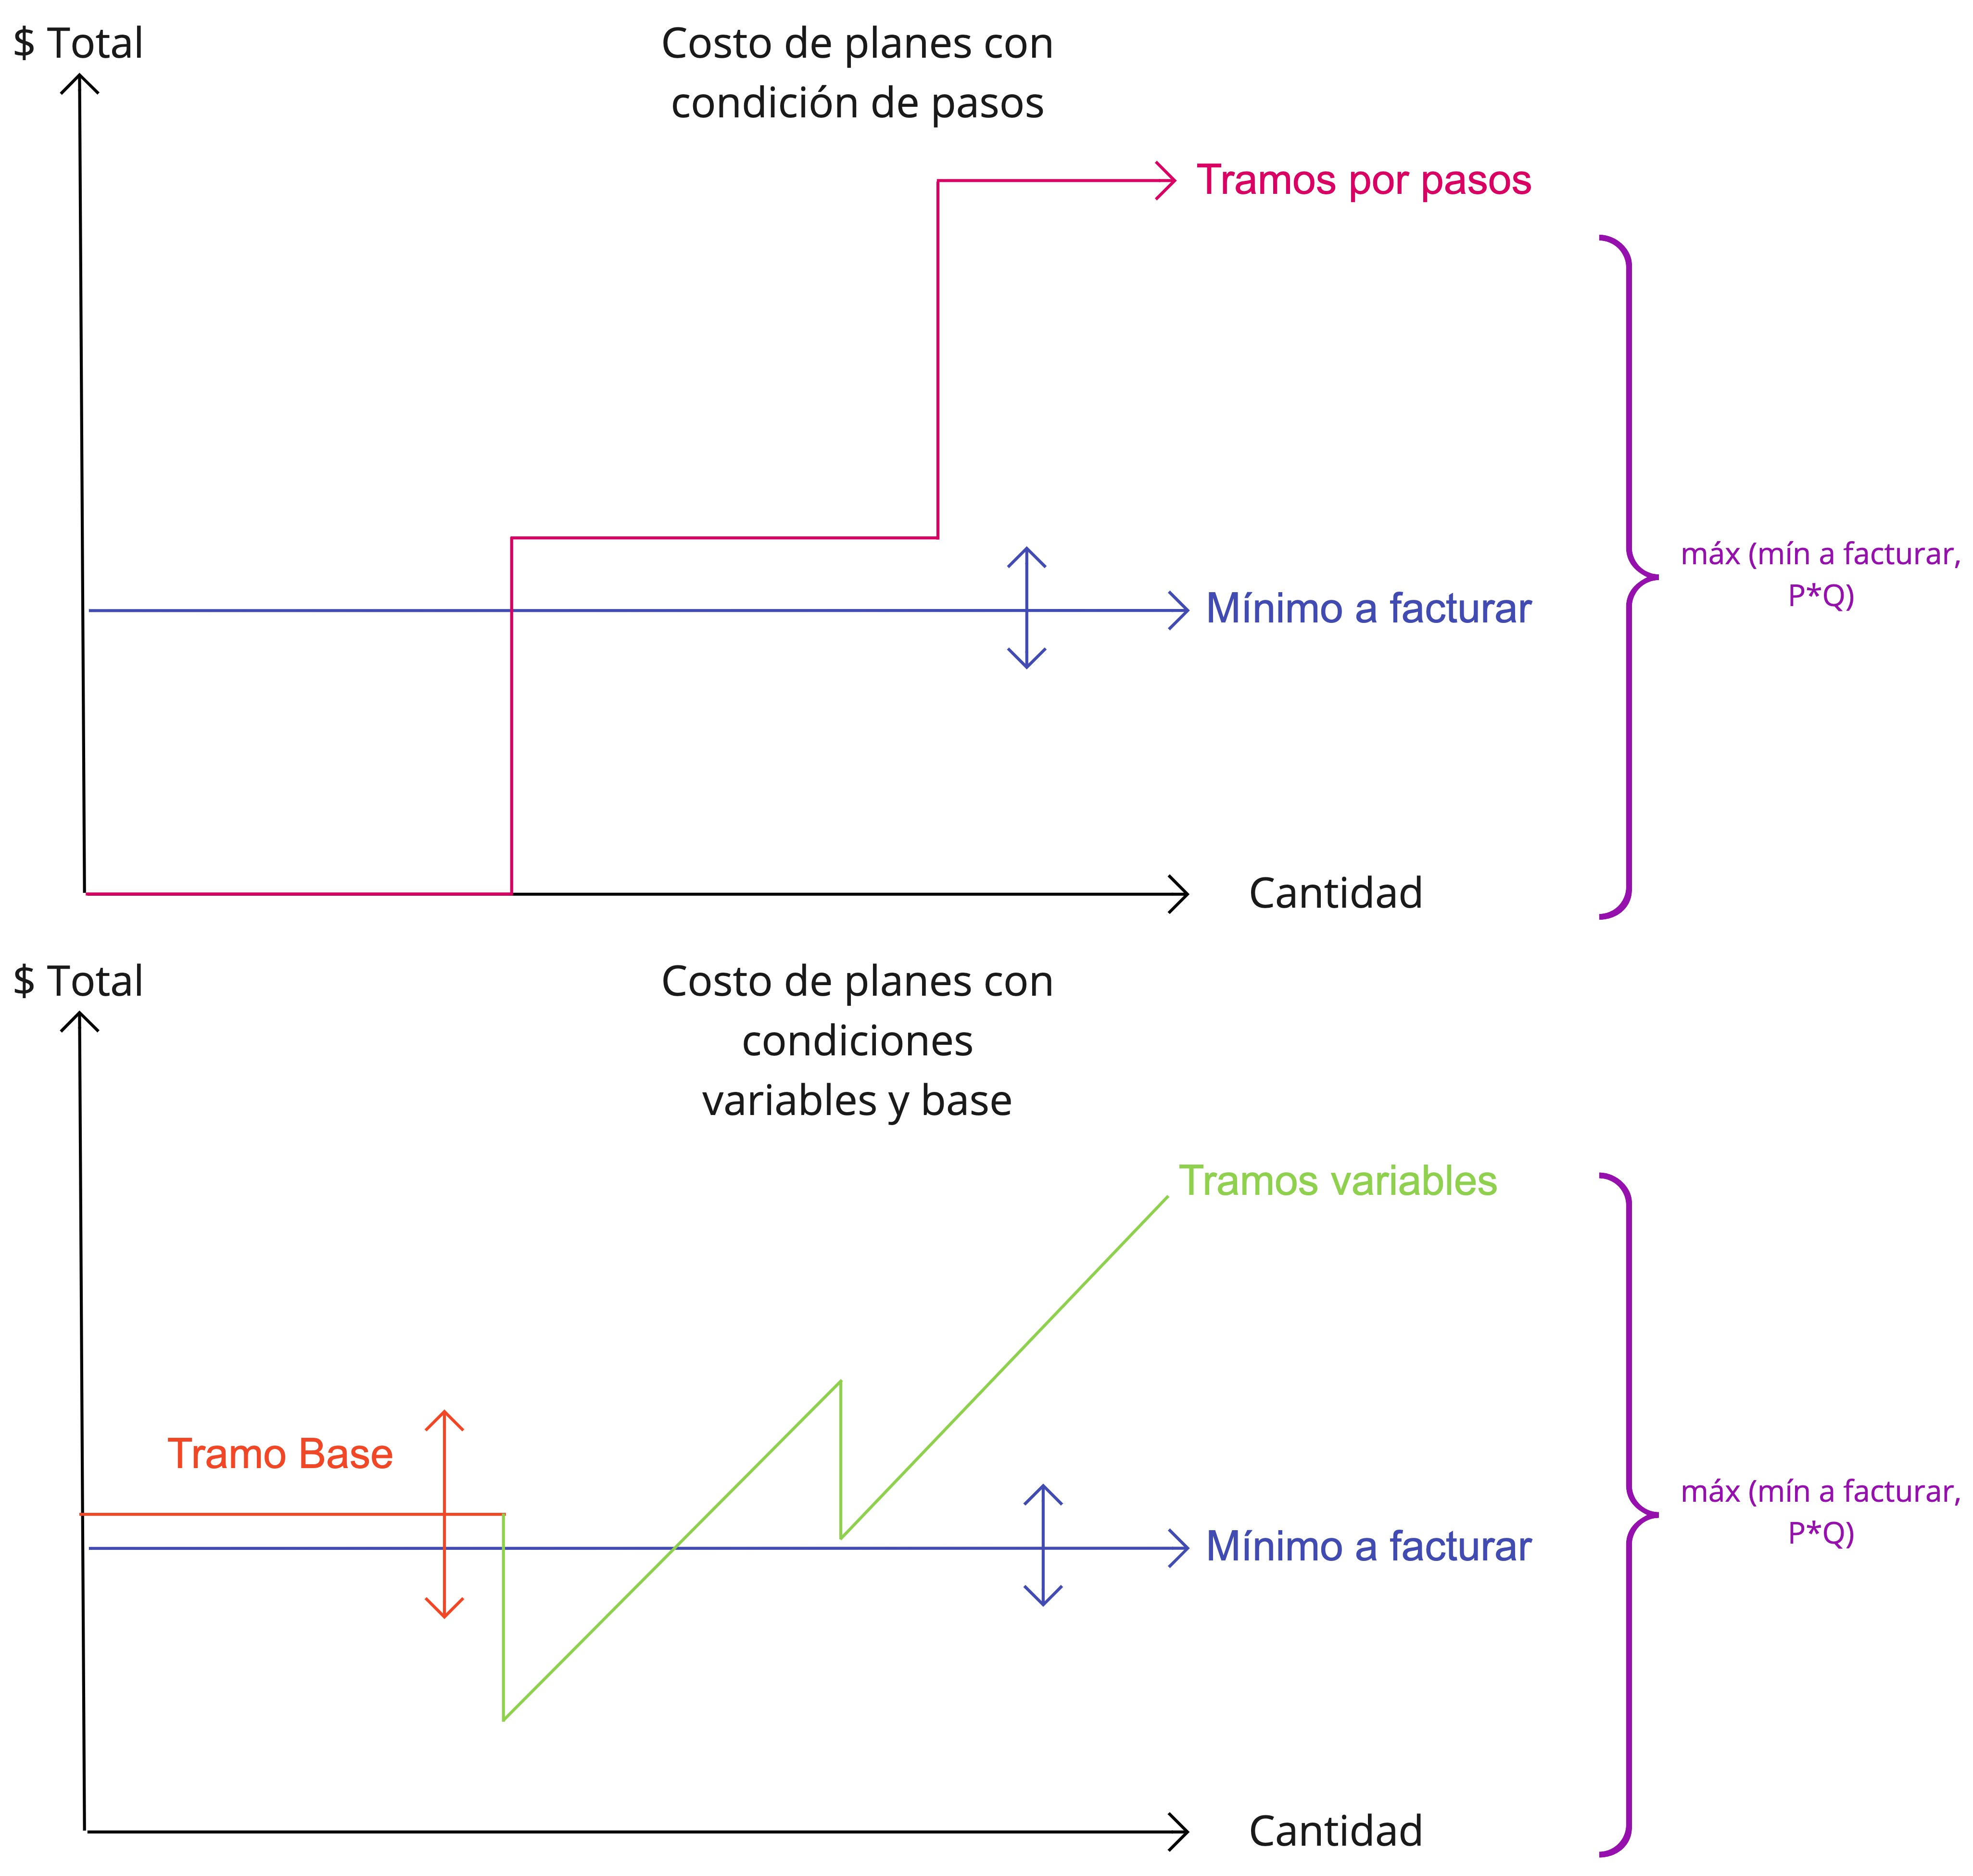
\includegraphics[width=0.6\linewidth]{figures/cc/cc_pricing_chart.jpg}
      \caption{Modelos de cobros y condiciones comerciales.}
      \label{fig:cc_pricing_chart}
    \end{figure}

    En segundo lugar, el modelo de relación plan (\texttt{plan\_relations}) tiene el rol de asociar el contrato del cliente con el plan creado de manera desacoplada y permitiendo la reutilización de planes estándares. 
    
    En tercer lugar, ``\texttt{plan\_relation\_proposals}'' tiene el propósito de permitir que se pueda tener una agrupación de relaciones de planes en un mismo modelo en caso de que un vendedor haya pactado con un cliente condiciones no estándar. Las condiciones estándar se definieron en conjunto con los vendedores a lo largo de múltiples reuiones y una posterior validación de Felipe Porter, jefe del área de ventas de la empresa. En caso de que las condiciones que un vendedor no sean las predefinidas y acordadas se definió que estas requerirían aprobación de Felipe Porter o Sebastián Ojeda (CEO). En caso contrario, las condiciones para el cliente determinado se aprueban de manera automática y se pueden utilizar al momento de facturar.
    
    En cuarto y último lugar el modelo ``\texttt{comments}'', tiene el propósito de simplemente contener el cuerpo del comentario por parte del vendedor en caso de que quiera hacer notar algo de los planes que está creando.

    En la figura \ref{fig:cc_relations} se puede observar los diferentes modelos y sus relaciones, junto con sus campos y tipos de datos por campo.
    
    \begin{figure}
      \centering
      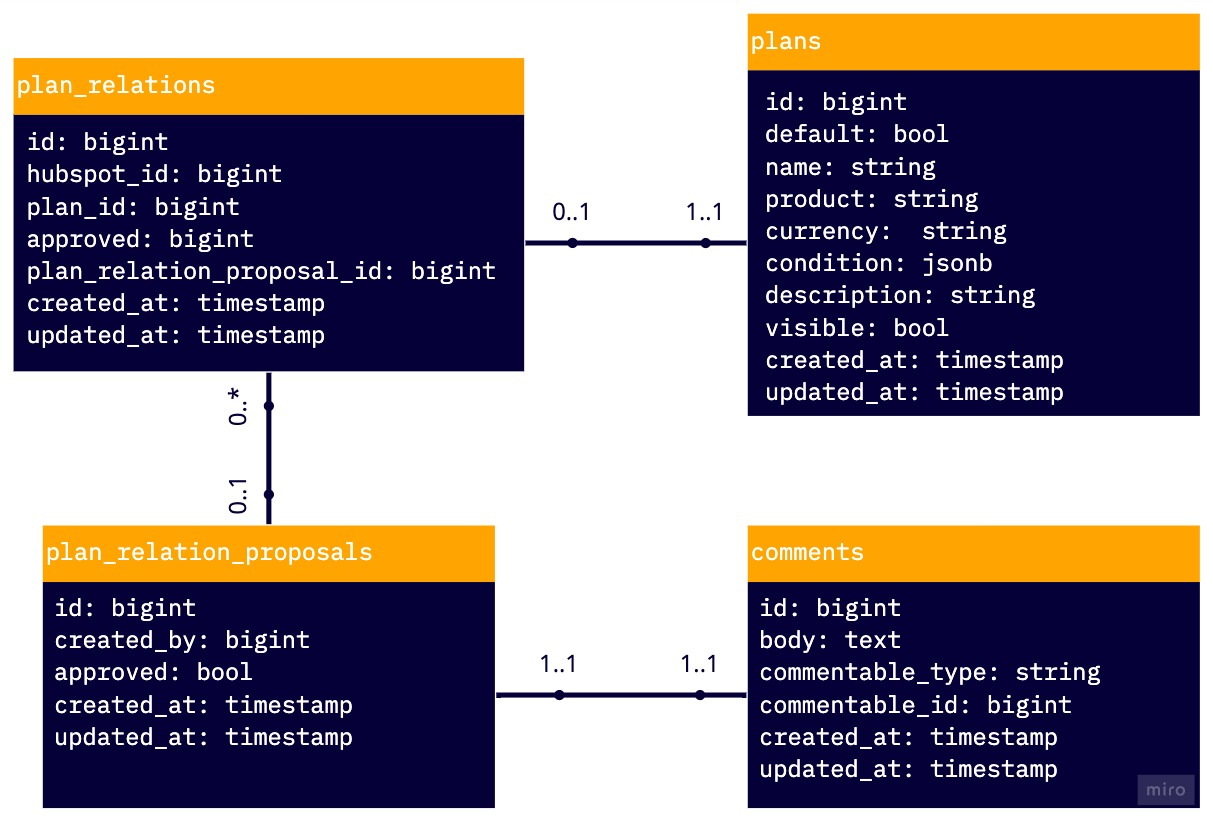
\includegraphics[width=0.75\linewidth]{figures/cc/cc_relations.jpg}
      \caption{Relaciones de modelos de condiciones comerciales.}
      \label{fig:cc_relations}
    \end{figure}

  \subsection{\textit{Solver} de condiciones y arquitectura}

    El paso siguiente a la creación de los modelos a utilizar, fue el de la creación de un módulo dentro del servicio de condiciones comerciales  que permitiese calcular la facturación adecuada para un cliente en específico dado el uso que este tuvo durante el mes. El módulo de cálculo se basa en un servicio específico para cada producto existente dentro de la empresa, es decir, por cada producto se tiene un servicio específico para calcular y resolver el cobro a realizar para ese producto dado el uso entregado.

    La información externa que el servicio de cálculo requiere es el identificador del cliente, junto con el uso de los productos. Al momento de hacer el llamado al servicio, este, con la información entregada, se programó de manera de que pase por una calculadora genera y delegador, de manera de que se subdelegue el cálculo del monto a facturar por cada producto a los subservicios específicos por productos. Este último diseño se basó en la implementación del patrón de diseño ``mediador'', en el cual se restringe las comunicaciones directas entre los objetos, forzándolos a colaborar únicamente a través de un objeto mediador \cite{pattern_mediator} y ``fachada'', en el cual se proporciona una interfaz simplificada a una biblioteca \cite{pattern_facade}. Por otro lado, la información del tipo de cobro se obtiene directamente desde la base de datos del servicio mediante el producto que se quiere calcular y el identificador del cliente para el cual se está calculando.
    
    Una vez que se realizó el cálculo por producto, el servicio retorna la información a un método que agrupa los diferentes resultados, suma el total y entrega un desglose por producto y por moneda, especificando el servicio de resolución utilizado, junto con la glosa a utilizar al momento de generar la factura en el ERP. En la figura \ref{fig:cc_calculator} se puede ver de manera general el flujo utilizado en el \textit{solver} y calculadora de costos.

    \begin{figure}
      \centering
      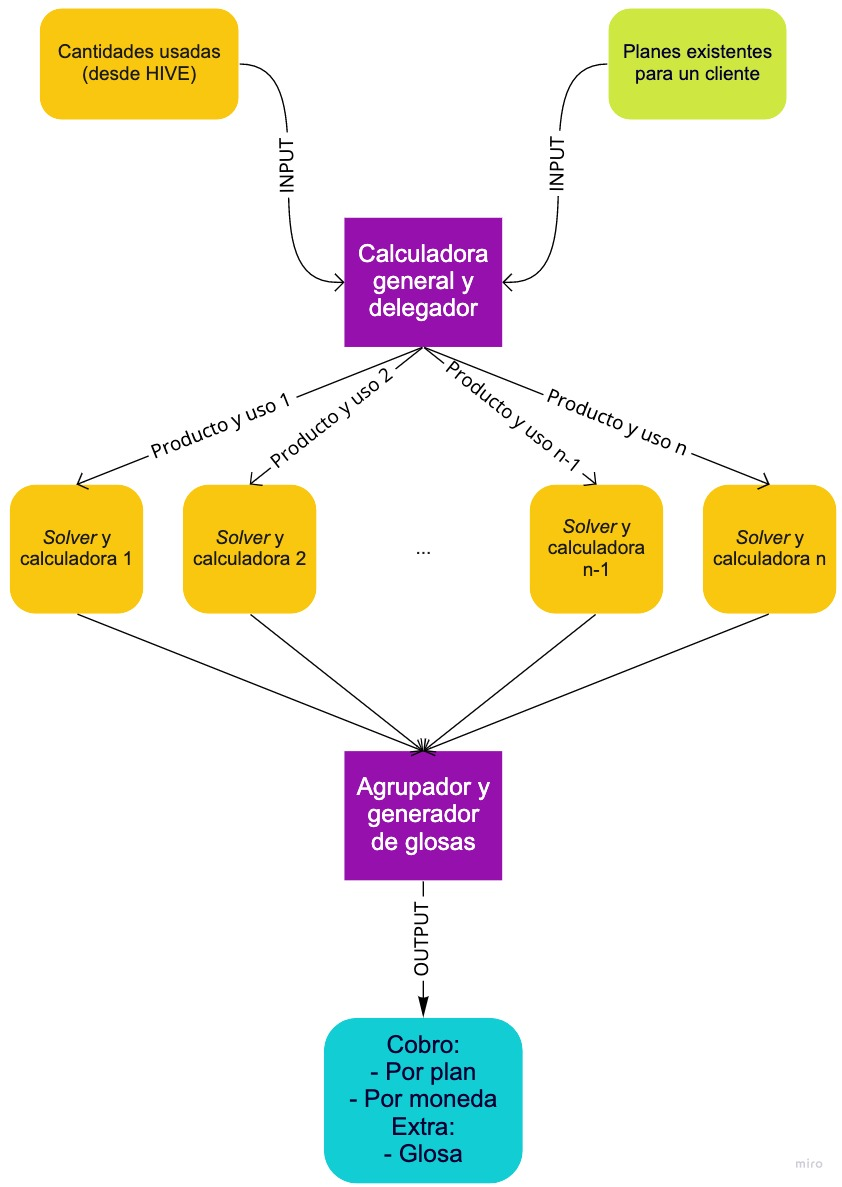
\includegraphics[width=0.5\linewidth]{figures/cc/cc_calculator.jpg}
      \caption{Esquema de delegación de \textit{solver} y calculadora.}
      \label{fig:cc_calculator}
    \end{figure}


    Posteriormente, una vez realizado el servicio de cálculo, se procedió a conectar el ERP con el servicio de condiciones comerciales. Para realizar la conexión se optó por utilizar una API con GraphQL expuesta por parte del servicio de condiciones comerciales. Por parte de \textit{Hive}, se utilizó Artemis, una librería de RoR que permite conectar el cliente, en este caso el ERP, con la API de manera casi invisible, exponiendo los métodos como si fuesen nativos de la aplicación \cite{artemis_gem}. Esta implementación permite a su vez que otras aplicaciones dentro de Beetrack consuman el servicio mediante el ERP, en caso de ser requerido. En la figura \ref{fig:cc_arquitectura} se puede observar la arquitectura con los dos \textit{pods} diferentes de GKE, uno para el ERP y otro para el servicio de condiciones comerciales y su comunicación mediante una API con GraphQL.

    \begin{figure}
      \centering
      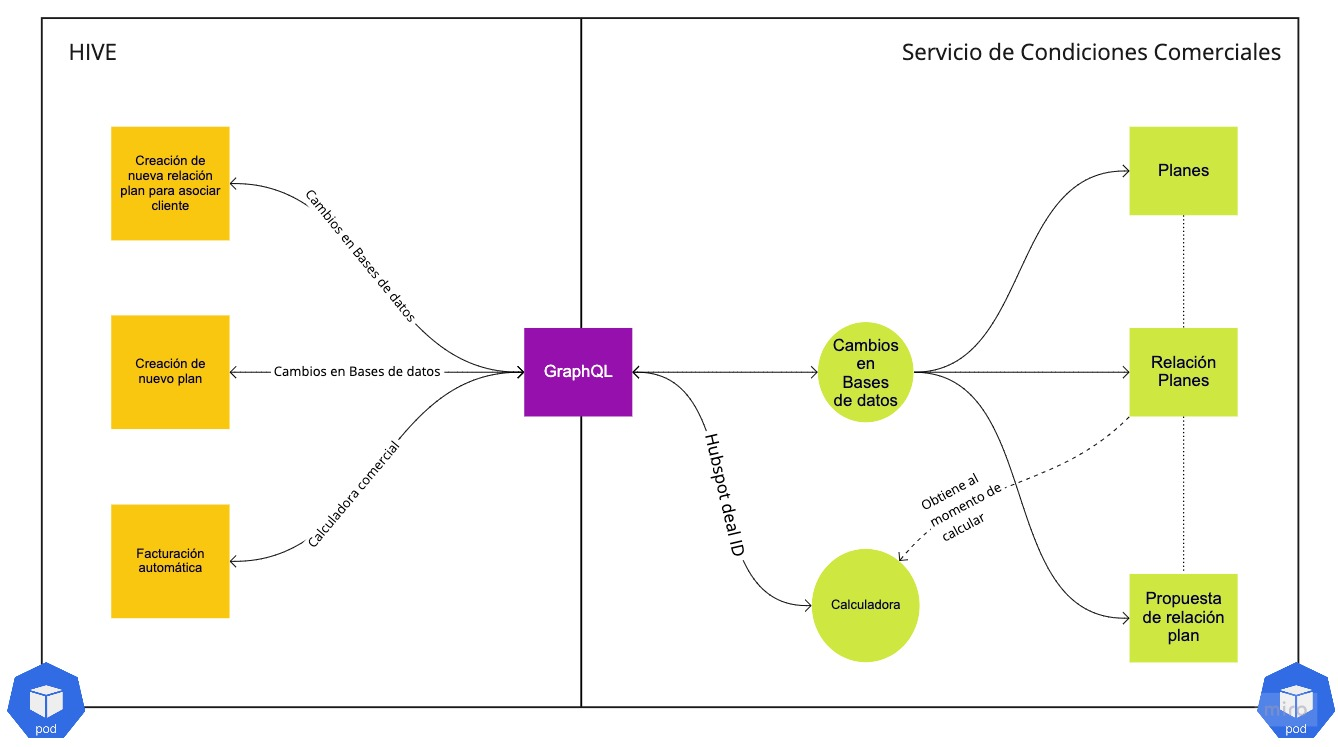
\includegraphics[width=\linewidth]{figures/cc/cc_arquitectura.jpg}
      \caption{Relaciones de modelos de condiciones comerciales.}
      \label{fig:cc_arquitectura}
    \end{figure}
    
  \subsection{\textit{Refactoring} y generación de facturas automáticas}

    Una vez que el alumno conectó el servicio de condiciones comerciales al ERP, este procedió a desacoplar el sistema antiguo que generaba las facturas de manera automática los 28 de cada mes. Esto se hizo en favor del servicio nuevo externo a \textit{Hive}, adaptando el código antiguo al sistema nuevo permitiendo un desacoplamiento de la lógica por parte del ERP, delegándosela al sistema creado. Este cambio implicó la eliminación de más de mil líneas de código en el ERP, con cosas tales como la generación de glosas y cálculo de montos a facturar.

    Posteriormente, el alumno le pidió al CEO de la empresa, Sebastián Ojeda, el archivo de Excel en el cual mantenía las condiciones comerciales de manera de poder poblar el servicio. Para esto, el alumno se comprometió a no entregar los datos de facturación a nadie sin autorización previa, manteniendo un código ético intachable dada la sensibilidad de los datos. Adicionalmente, dado que el elevado número de contratos de la empresa (mayor a 500), se decidió escribir código que transcribiese el archivo excel al formato del servicio, generando más de 1500 planes diferentes válidos.

    Luego de que se transcribieran los planes generados al servicio de condiciones comerciales, el alumno se coordinó con el equipo de \textit{Data Science} de manera de poder hacer simulaciones de facturación antes de poner en funcionamiento el servicio de generación de facturas reales. De esta manera, se simuló una ejecución del problema real y se puso a prueba el código desarrollado para tener conocimiento de cuán preciso era. El alumno trabajó con el equipo de \textit{Data Science}, dado que este es el encargado de la carga de datos de uso de los clientes, por lo que se pudo generar simulaciones con diferentes niveles de uso y para diferentes clientes. Los resultados obtenidos fueron altamente prometedores, obteniendo aproximadamente una precisión de facturación del orden de 87,9\%. Finalmente, el 28 de octubre corrió el servicio de generación automática de pre-facturas exitosamente y recibió comentarios muy positivos por el equipo contable de la empresa, dado que no tuvieron que modificar las pre-facturas antes de emitirlas.

  \subsection{Creación de condiciones por parte de vendedores y aprobación de gerentes}
    En paralelo junto con la generación automática de pre-facturas, el alumno trabajó en 4 vistas dentro del ERP, las cuales correspondían a dos formularios y dos vistas generales. Adicionalmente se crearon 3 plantillas de correos mediante HTML, CSS y Ruby embebi; estas se detallarán más adelante. Estas vistas fueron validadas y diseñadas junto a Grace Lillo, del equipo de \textit{design ops}, de manera de que estas fueran realmentes útiles para los usuarios finales. Cabe mencionar que estas vistas fueron generadas utilizando los componentes de \textit{Honeypot} en React. 
    
    % vista general de condiciones comerciales
    En primer lugar, el estudiante programó una vista general en donde los vendedores pueden ver las condiciones comerciales preaprobadas por los gerentes, de manera de poder tener una noción de cuáles son las condiciones de cada plan antes de utilizarlo para un determinado cliente. A continuación, en la figura \ref{fig:cc_visible}, se puede ver la vista mencionada anteriormente.

    \begin{figure}[H]
      \centering
      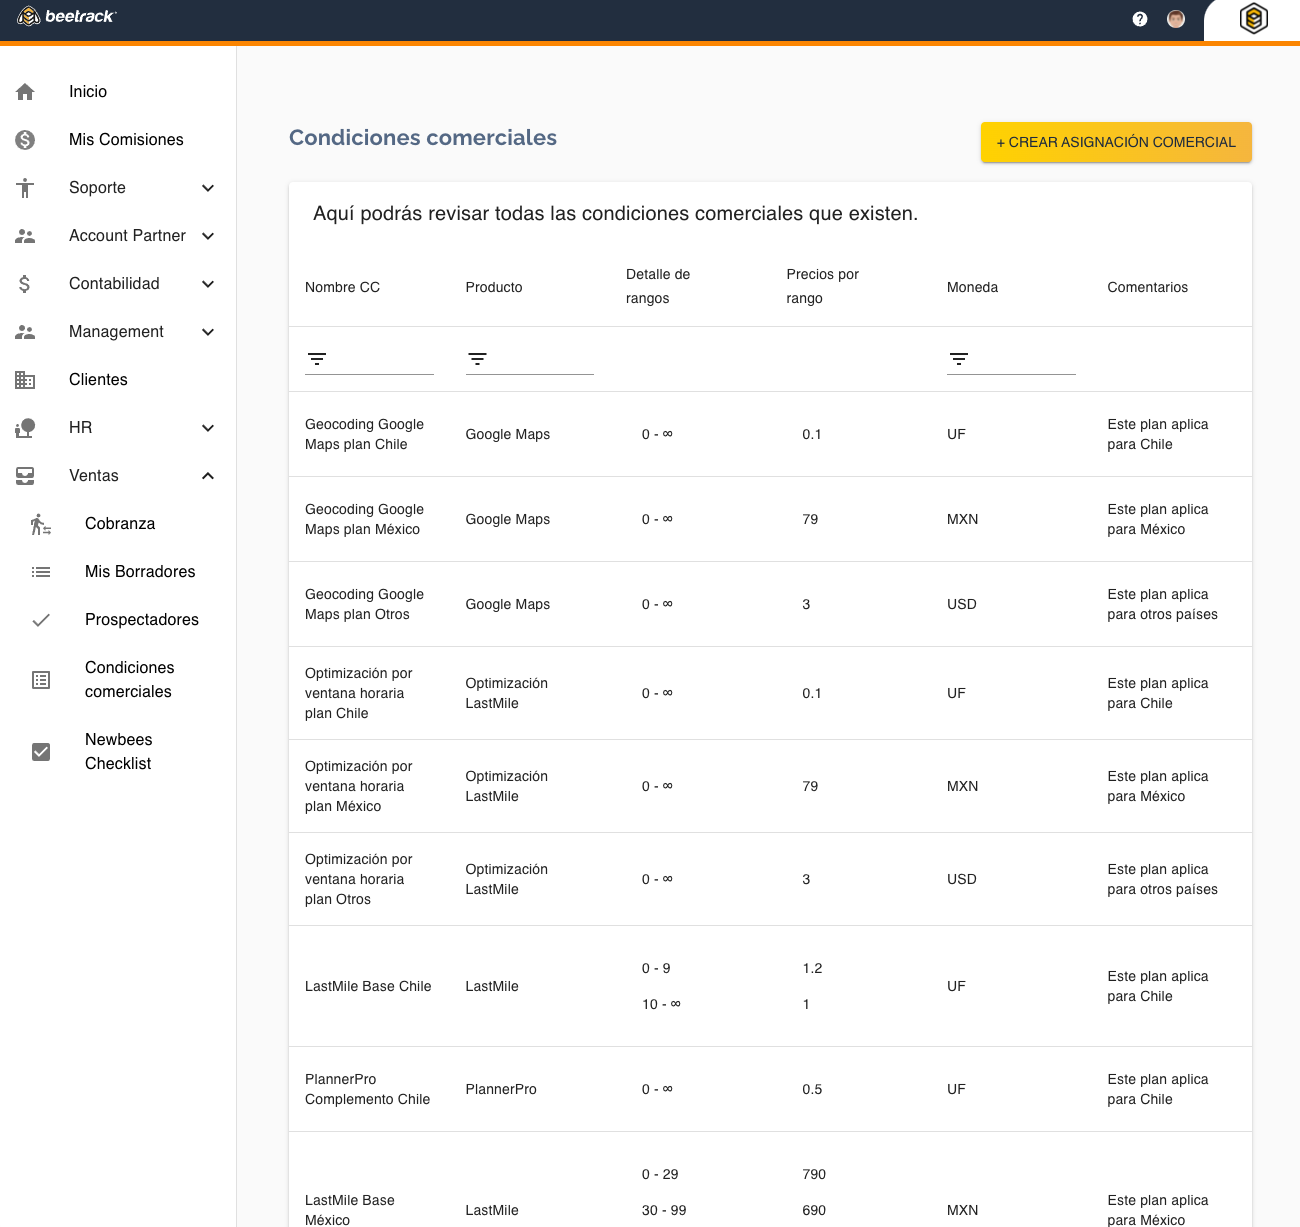
\includegraphics[width=0.6\linewidth]{figures/cc/vistas/cc_visible.png}
      \caption{Vista general de condiciones comerciales preaprobadas.}
      \label{fig:cc_visible}
    \end{figure}

    % vista de creacion de condicion comercial nueva por vendedor
    En segundo lugar, el alumno realizó una formulario que le permite a los vendedores crear asociaciones comerciales, es decir, asociar una condición comercial existente y preaprobada a un cliente determinado. Parte crucial del formulario es el hecho de que se puedan definir precios distintos y montos mínimos a facturar solamente para los productos y no para los servicios, ya que esto va en línea con el plan de la empresa de tener planes estandarizados y asimilarse más a un SaaS tradicional. 
    
    Un punto importante de este flujo es el hecho de que si el vendedor cambia el precio predefinido del tramo de un producto, entonces se notificará mediante un correo como el de la figura \ref{fig:cc_mail_new} a los gerentes de esta propuesta, de manera de que esta propuesta pueda ser aprobada o rechazada. En caso de que el plan preaprobado no tenga cambios en los precios, este se aprobará de manera automática. Lo anterior fue un pedido específico por parte de los gerentes con el propósito de de poder tener mayor control sobre los tipos de planes que crean los vendedores para así evitar la generación de planes poco comunes. 
    
    El formulario mencionado se puede ver en la figura \ref{fig:cc_new_sales_man}.

    % vistas de nueva condicion comercial y mail
    \begin{figure}[H]
      \centering
      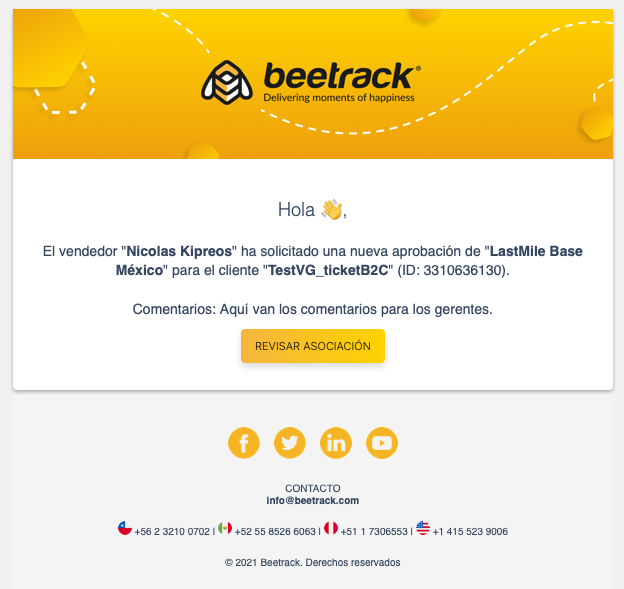
\includegraphics[width=0.6\linewidth]{figures/cc/mails/cc_mail_new.png}
      \caption{Correo electrónico de solicitud de aprobación de asociación comercial.}
      \label{fig:cc_mail_new}
    \end{figure}

    \begin{figure}[H]
      \centering
      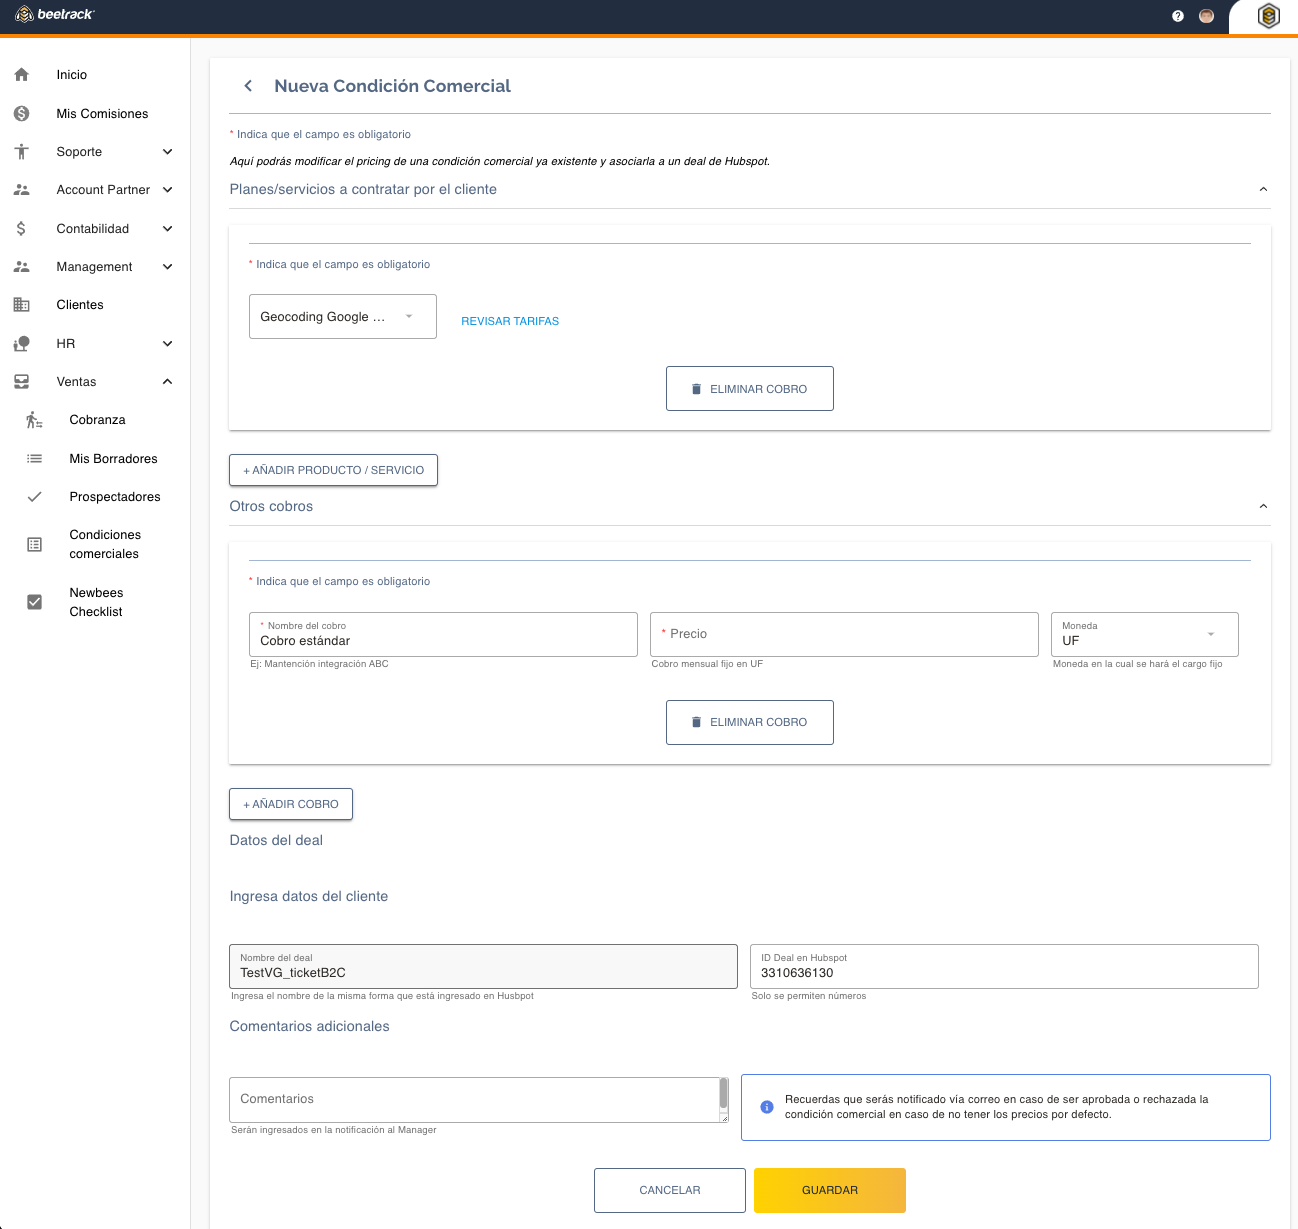
\includegraphics[width=0.6\linewidth]{figures/cc/vistas/cc_new_sales_man.png}
      \caption{Vista general de condiciones comerciales preaprobadas.}
      \label{fig:cc_new_sales_man}
    \end{figure}

    % vista de creacion de aprobacion de condicion comercial
    En tercer lugar, el alumno programó una vista para los gerentes en la cual estos pueden aprobar o rechazar las propuestas de asociaciones comerciales creadas con precios no estándares. Esta vista se puede ver en la figura \ref{fig:cc_review}. Una vez que los gerentes aprueben o rechacen la propuesta, esto se le notificará al vendedor correspondiente el correo correspondiente de la figura \ref{fig:cc_approve_reject}.

    \begin{figure}
      \centering
      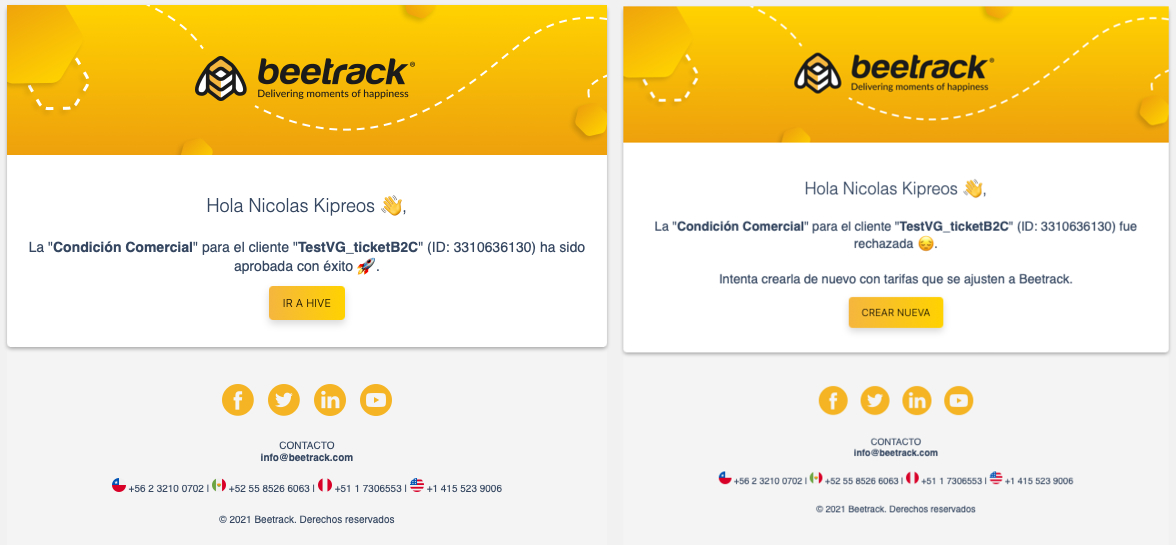
\includegraphics[width=\linewidth]{figures/cc/mails/cc_approve_reject.jpeg}
      \caption{Correo electrónico de aprobación (izquierda) y rechazo (derecha) de asociación comercial.}
      \label{fig:cc_approve_reject}
    \end{figure}

    \begin{figure}[H]
      \centering
      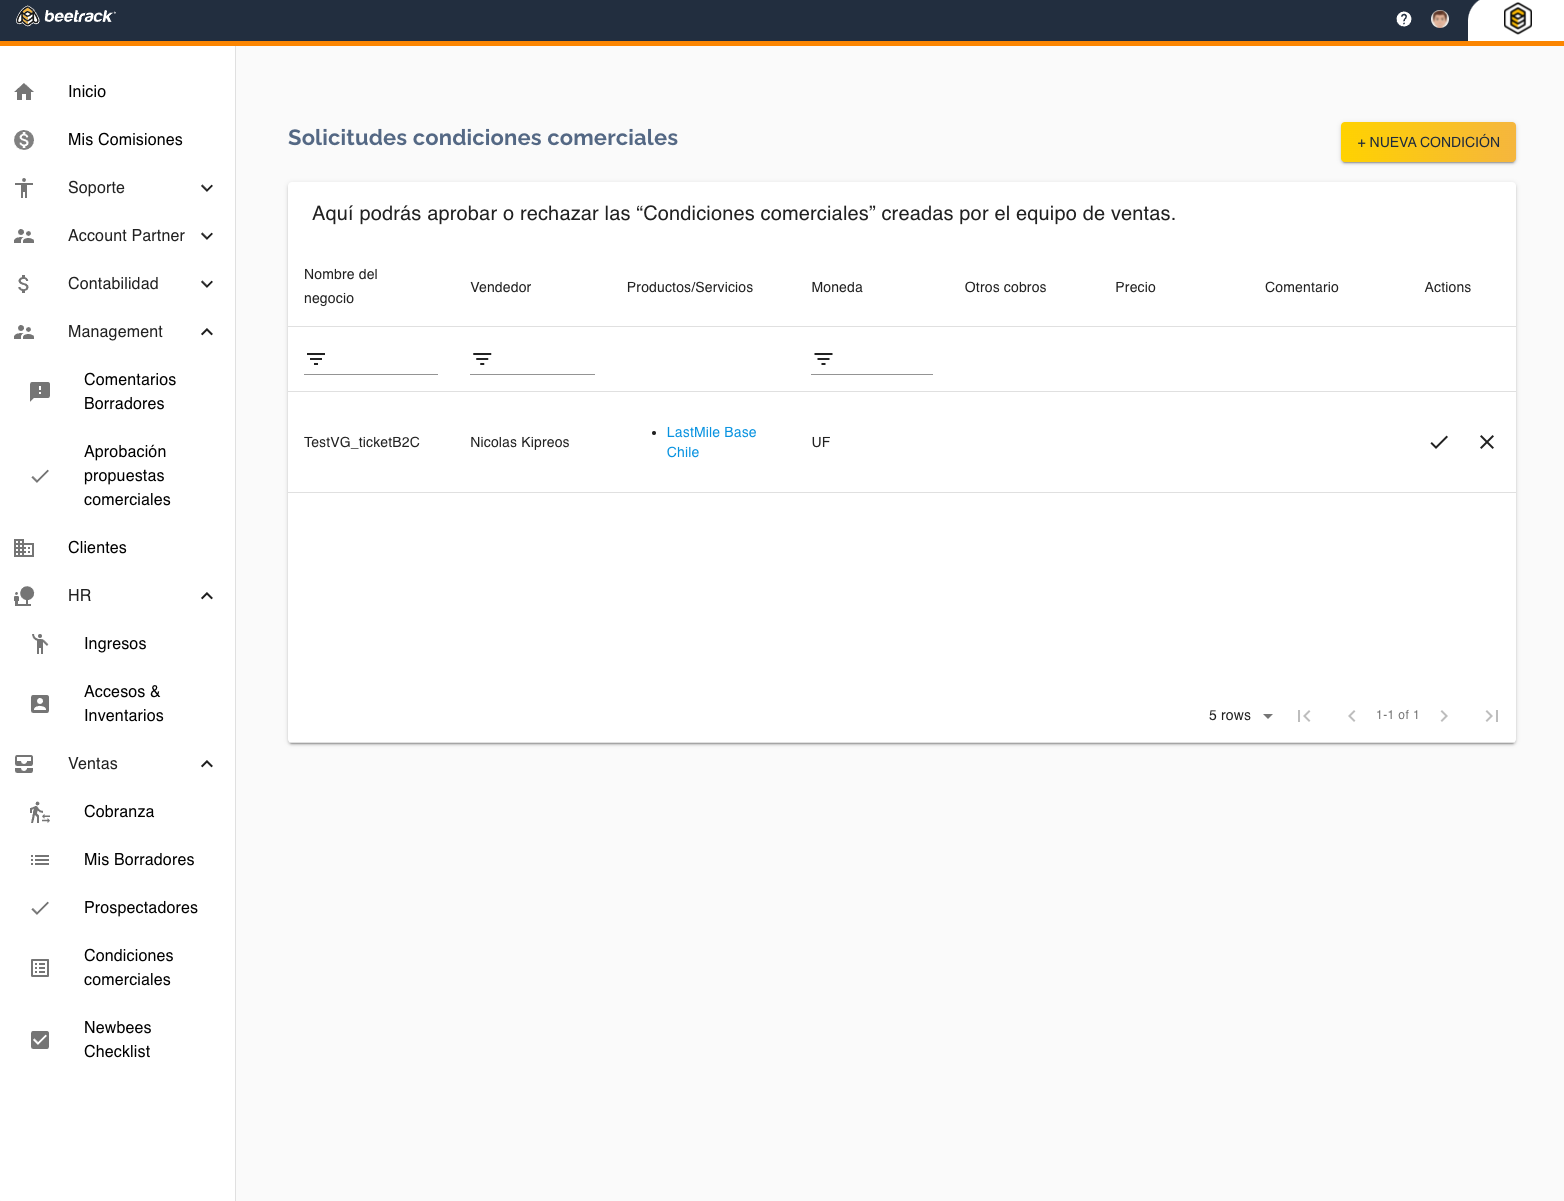
\includegraphics[width=0.6\linewidth]{figures/cc/vistas/cc_review.png}
      \caption{Vista de aprobación y rechazo de asociaciones comerciales.}
      \label{fig:cc_review}
    \end{figure}

    % vista de creacion de condicion comercial nueva desde cero por gerente

    En cuarto, y último luar, se realizó un formulario totalmente personalizado para la creación de planes no estandarizados, tanto para productos como servicios. Este formulario solo es accesible por los vendedores, sino que solamente los genertes tienen acceso. El propósito de este formulario es poder crear un plan totalmente a medida para un cliente en caso de que un plan estándar no permita abarcar el tipo de contrato que se cerró. Esta decisión de restricción del formulario a los gerentes se generó principalmente para evitar el fomentar que los vendedores vendan el producto de manera no estandarizada y Beetrack se pueda acercar más a un SaaS tradicional. En la figura \ref{fig:cc_new_manager} se puede observar el formulario descrito anteriormente.
 
    \begin{figure}[H]
      \centering
      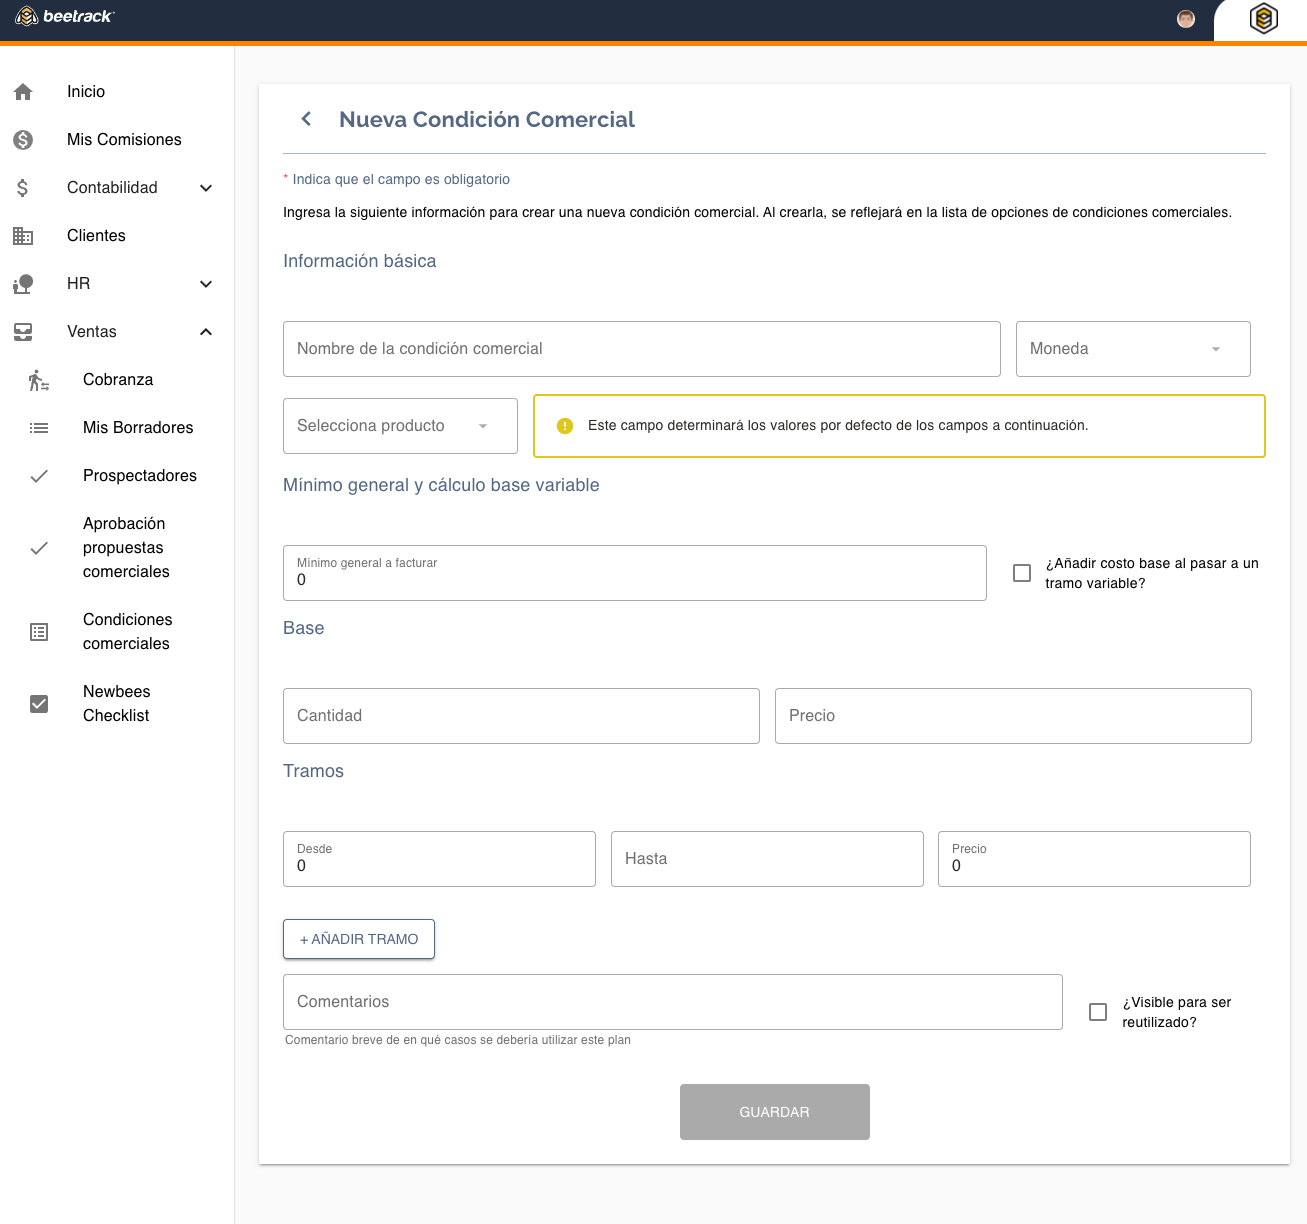
\includegraphics[width=0.6\linewidth]{figures/cc/vistas/cc_new_manager.png}
      \caption{Vista general de condiciones comerciales preaprobadas.}
      \label{fig:cc_new_manager}
    \end{figure}

\section{Resultados}

  Los resultados obtenidos para este proyecto estuvieron por sobre lo esperado en un comienzo. En particular se logró lo siguiente:

  \begin{enumerate}
    \item Servicio independiente de \textit{Hive}.
    
    Se creó un servicio independiente del ERP, que permitirá que se tenga la información descentralizada y se pueda enfocar en su única función de cálculo de costos y almacenamiento de planes de los clientes con tecnologías que no habían sido utilizadas dentro de la empresa anteriormente (GraphQL).

    \item Creación de modelos de planes flexibles.

    Se logró diseñar modelos de planes y condiciones lo suficientemente flexibles de manera que abarcaran a todos los casos existentes y por existir. Junto a esto, la forma en que se abarcó el campo ``\texttt{condition}'' del modelo perimitió tener un \textit{solver} flexible que se adaptase a la forma de resolver el csoto de los planes de manera correcta. Esta flexibilidad se logró mediante al trabajo entre múltiples áreas de la empresa, con especial foco en operaciones y ventas de manera de que se pudiese entender de mejor manera el problema y dolor existente. El esquema del modelo se logró definir gracias a un \textbf{análisis sistemático de los problemas} de los usuarios y trabajo en conjunto con las diferentes áreas de la empresa.

    \item Servicio con 87,9\% de precisión de facturación.
    
    Se creó un servicio de resolución de condiciones comerciales independiente del estado de los clientes, que permite calcular el costo asociado al uso de cada cliente, por producto, por servicio y por moneda. Esto permitió que se tenga una facturación mucho más precisa que otros intentos para la resolución de este problema, subiendo en más de un 40\% la precisión de la facturación de más de 500 facturas desde el último intento que fue en Hubspot con una precisión de 43\%. Esto se pudo lograr mediante una batería de \textbf{simulaciones de soluciones} y aplicación de \textbf{conocimientos avanzados de ingeniería de software} de manera de crear un \textit{software} escalable mediante diferentes patrones de diseño.

    \item Formularios de creación de condiciones.

    El alumo programó las vistas de \textit{frontend} dentro de \textit{Hive} mediante el diseño en conjunto con \textit{design ops}, resultando en los formularios especializados para los vendedores y el totalmente personalizable para los gerentes. Estos formularios quedaron \textbf{expresados en JavaScript} en el \textit{framework} de React.
    
    \item Vista de aprobación.
    
    Se desarrolló una vista especializada que permite que los gerentes de la empresa aprueben o rechacen las propuestas de asociaciones comerciales creadas por los vendedores en caso de que no sean tengan valores preaprobados. El objetivo de esta vista es poder tener una visión rápida de lo que están haciendo los vendedores de la empresa y también poder tener un control fino de qué tipos de condiciones comerciales se tiene para los clientes.
    
    \item Correos de estado propuestas comerciales.
    
    Se crearon 3 correos automáticos que se envían en diferentes momentos acorde a los cambios de estado que ocurran para los planes y para las propuestas de de asociaciones comerciales.

  \end{enumerate}

\chapter{Conclusiones} \label{conclusiones}
\section{Competencias evidenciadas}

  El trabajo realizado por el alumno como ingeniero de \textit{software}, en Beetrack durante los cuatro meses evidencian de manera clara cada una de las tres competencias declaradas del perfil. En específico se pudo evidenciar lo siguiente:

  \begin{enumerate}
    \item Aplicar conocimientos avanzados de Ciencia de la Computación, Ingeniería de Software y Sistemas de Información para entender problemas complejos y abiertos.
    
    El estudiante desarrolló un sistema especializado con una arquitectura de software diseñada para ser escalable y replicable rápidamente mediante el uso de tecnologías como GKE y contenedores de Docker, como también hizo uso avanzado de del \textit{frmework} RoR utilizando validadores personalizados en los modelos. Adicionalmente, el estudiante utilizó de manera amplia el \textit{framework} de pruebas RSpec, lo que implica un uso de buenas prácticas de \textit{software} que lo permite hacer más escalable, predecible y estable.

    Por otro lado, para poder diseñar de manera adecuada los aparatos de \textit{software} creados, el estudiante tuvo que aplicar conocimiento teórico de patrones avanazdos de diseño, de manera de que se pudiese tener un código altamente cohesivo y con bajo acoplamiento, algo que es sumamente deseado. Para poder abordar los dos puntos mencionados anteriormente, el estudiante tuvo que comprender las diferentes problemáticas del problema y utilizar sus conocimientos en las diferentes áreas para abarcarlos.

    Finalmente, el estudiante tuvo que utilizar conocimientos de sistemas de información, tales como la lógica de negocio de un ERP, que fue en lo que el alumno trabajó. Esto se traduce directamente en la combinación e integración que se realiza con Hubspot y Quickbooks, junto con el uso que \textit{Hive} le da a nivel de lógica de negocio.

    \item Diseñar y desarrollar modelos y artefactos de software y simular soluciones a problemas de la Ciencia e Ingeniería de Computación, cumpliendo con restricciones técnicas, sociales y éticas.
    
    Por un lado esta competencia se puede ver evidencada mediate el aumento sistemático del nivel de cobertura de código del ERP. Esto se debe a que las pruebas automatizadas son una forma de simulación de ejecución del código en un ambiente aislado, solucionado el problema de confiabilidad y resiliencia ante fallas del código. En este sentido, el alumno logró diseñar artefactos de \textit{software} que simularan la ejecución del mismo código escrito, manteniendo resguardada información sensible de otros entornos.

    Por otro lado, esta competencia también se pudo ver evidencada las simulaciones de la emisión de pre-facturas y cáluclo de uso por parte de los clientes. Esto se debe a que para poder tener seguridad de que el servicio programado tenía una mayor precisión que los sistemas anteriores se tuvo que realizar simulaciones de uso de manera de no itervenir los datos reales. A su vez, esto implicó restricciones sociales y éticas al no poder compartir la información de facturación real con nadie más dada la naturaleza de la tarea, mientras que al mismo tiempo se logró un incremento de casi un 50\% en términos de precisión de facturación.

    Adicionalmente, se desarrolló modelos y artefactos de \textit{software} mediante la creación de los modelos que el servicio de condiciones comerciales aloja (\texttt{plans}, \texttt{plan\_relations}, \texttt{plan\_relation\_proposals} y \texttt{comments}), como también los artefactos que permiten el cálculo correcto de los montos acorde a los modelos generados. Cabe mencionar que los artefactos generados también cumplen con restricciones técnicas en cuanto al hecho de no mantener registros del resultado final, delegando esa tarea al ERP, dado que \textit{Hive} es el sistema que genera la factura real y mediante el cual se realizan los cobros a los clientes.

    \item Analizar en forma sistemática las diferentes problemáticas de los usuarios, y diseñar productos o sistemas de software que queden expresados mediante algún lenguaje de programación, de acuerdo a los estándares de la ingeniería de software.
    
    Esta competencia se pudo ver evidencada por las diferentes etapas del levantamiento del servicio de condiciones comerciales: modelamiento, creación de un \textit{solver} y generación de vistas.
    
    Para la etapa de modelamiento se analizó la necesidad de migrar las condiciones comerciales a un servicio especializado que tuviese un esquema y modelamiento flexible de manerar de que abarcara todos los planes existentes y los futuros. Esta problemática fue identificada dado el tamaño de la empresa y el hecho de que las condiciones comerciales no habían logrado ser abarcadas de manera correcta en dos intentos anteriores y se resolvió con los esquemas planteados en la sección \ref{modelamiento}. Este paso quedó plasmado en el leguaje Ruby montado sobre el \textit{framework} Rails.

    Para la segunda etapa, se identificó la problemática del traspaso del cálculo de facturación mediante un archivo excel no escalable como un dolor por parte de la empresa y del área contable de esta. La solución a este problema se ve evidenciada mediante la creación de un \textit{solver} generalizado que se adecue dependiendo de las condiciones comerciales de cada cliente y cada producto, quedando expresado en RoR con un esquema de delegación con patrones de diseño como se puede observar en la figuras de la sección \ref{solver_y_arquitectura}.

    Finalmente, para la tercera etapa, se hizo notar por parte de los gerentes la necesidad de acotar los campos editables por los vendedores, por lo que el alumno, junto con Grace Lillo, diseñaron los formularios de creación de condiciones comerciales acorde a lo planteado. Adicionalmente, se relizaron validaciones con todas las partes involucradas, de manera de que se asegurara el resolver el dolor de todos. Esta solución de formulario de creación de condiciones comerciales quedó expresada en el \textit{framework} React en el lenguaje JavaScript.

  \end{enumerate}

\section{Conclusiones generales}

  Acorde a lo trabajado durante cuatro meses por el alumno en Beetrack, se puede afirmar que se cumplieron las tres competencias planteadas inicialmente en la sección \ref{competencias} fueron ampliamente validadas. Para lograr las metas y competencias propuestas, el alumno se desempeñó como Ingeniero de \textit{Software full-stack} dentro del área de operaciones en Beetrack.
  
  Los proyectos que el alumno llevó a cabo dentro del equipo de operaciones fuero dos: la creación de un servicio de concidionces comerciales  y el aumento sistemático de la cobertura de pruebas automatizadas. El servicio creado le permitirá a la empresa tener una facturación mucho más precisa que antes, logrando un 87,9\% de precisión, mientras que al mismo tiempo le facilitará el tener servicios especializados para el cálculo del costo por uso de cada cliente para producto y que este cálculo se integre de manera simple con el ERP. Por otro lado, el incremento de cobertura por parte de las pruebas automatizadas le entregará una mayor seguridad a al equipo y a \textit{Hive}, mientras que al mismo tiempo se podrá detener la puesta en producción del código fallido de manera preventiva gracias a la integración continua que se realizó con Circle CI.

  Finalmente, el alumno tuvo la oportunidad de desempeñarse de manera profesional y pudo utilizar de manera amplia los conocimientos adquiridos durante sus años universitarios. Adicionalmente, el estudiante también logró desempeñarse de buena manera mediante un trabajo en equipo y con diferentes áreas, lo que le permitió también hacer uso de las habilidades blandas adquiridas en la carrera. La combinación del uso de habilidades blandas como conocimientos teóricos y prácticos permitieron que el alumno demostrara también un buen trabajo en equipo, resolución de problemas y soluciones innovadoras a problemas complejos mediante las herramientas adquiridas en la universidad.

%%%%%%%%%%%%%
%       REFERENCES        %
%%%%%%%%%%%%%

\cleardoublepage
\phantomsection \label{references}
\bibliographystyle{apacite}
\renewcommand{\bibname}{Referencias}

%%%% ACTIVAR SIGUIENTES 3 LINEAS SI POSTGRADO RECHAZA LA BIBLIOGRAFIA
%\setlength{\bibleftmargin}{0em}
%\setlength{\bibindent}{0em}
%\setlength{\bibitemsep}{1em}


\bibliography{Thesis}

%%%%%%%%%%%%
%      APPENDICES      %
%%%%%%%%%%%%

% \appendix % It is like a chapter, so each appendix (A, B, C...) must to be considered as a section

% \newpage
% \section[First Appendix]{First Appendix}
% We can write equations here too:

\begin{equation}
\int_0^\infty e^{-x^2} dx
\end{equation}

And more...

% \newpage
% \section[An Interesting Short Story]{An Interesting Short Story}
% Let us enjoy reading this story of Hunting With The Lion. 

It was a dry summer. The animals in the forest were beginning to find it difficult to get food. 

A bear, a wolf and a jackal thought it would be better to join hands with a lion and do the hunting. They approached lion and he too agreed. The four of them went off hunting. 

The hunting party came across a buffalo. The fox and wolf chased the buffalo. The bear intercepted the buffalo. The lion killed him. 

The fox made shares out of the buffalo. When they were about to take their shares the lion roared and said, "Well friends, the first share is mine for my leadership. The second share is mine for, it is I who killed. The third share is also mine for I need it for my cubs. Anyone who needs a share can take the fourth. But before that you will have to win me.” 

All the three left the place without a single word. 

MORAL : {\bf If you are might, you are right}.

\end{document}
